%% ACM ISS 2026 Poster track -- REVIEW COPY with highlighted revisions (generated by
%% revision/make_highlighted.py from sigconf.tex; do not edit by hand, do not submit to TAPS).
%% Text follows the latest author revision (ISS2026_References_Last.pdf); every number,
%% method detail and quotation traces to "Main text.tex" or that revision.
%% ISS 2026 poster rules: at most 6 pages excluding references; double-column camera-ready.
\documentclass[sigconf]{acmart}

\AtBeginDocument{%
  \providecommand\BibTeX{{%
    Bib\TeX}}}

%% Rights management information.
%% OUTSTANDING: replace the next block with the exact commands from the ACM rights
%% confirmation email (\setcopyright, \acmDOI, \acmISBN, \acmBooktitle, ...), then set
%% printacmref=true. Nothing below is ACM-issued; conference name, dates and venue are
%% taken from the public ISS 2026 call.
\setcopyright{none}
\copyrightyear{2026}
\acmYear{2026}
\acmConference[ISS '26]{ACM Conference on Interactive Surfaces and Spaces}{November 23--26, 2026}{Turin, Italy}
\acmISBN{}
\acmDOI{}
\settopmatter{printacmref=false}

\graphicspath{{figures/}}
%% Lets TeX stretch interword space on lines it would otherwise leave overfull.
\emergencystretch=1em

\usepackage{pgfplots}
\usepackage{caption}
\usepackage{subcaption}
\usepackage{xcolor}
\pgfplotsset{compat=1.18}

%% Condition colours, matching the paper's figures.
\definecolor{numcue}{HTML}{3478D4}
\definecolor{iconcue}{HTML}{248C87}

%% ---- BEGIN REVISION MARKUP (review copy only; sigconf.tex is the clean source) ----
%% Highlights changes relative to the original ISS 2026 poster submission.
\usepackage{soul}
\definecolor{revhl}{HTML}{FFF3A3}
\sethlcolor{revhl}
\DeclareRobustCommand{\rev}[1]{\hl{#1}}
\DeclareRobustCommand{\revbox}[1]{{\setlength{\fboxsep}{0pt}\colorbox{revhl}{\strut #1}}}
\DeclareRobustCommand{\revcite}[1]{\revbox{\cite{#1}}}
\newcommand{\revcs}{\ }
\soulregister{\revbox}{7}
\soulregister{\revcite}{7}
\soulregister{\ref}{7}
\soulregister{\revcs}{0}
%% ---- END REVISION MARKUP ----

\begin{document}

\title[Reading a Remote Teammate's Body]%
{Reading a Remote Teammate's Body: A Body-Worn Sensing Interface for Group Coordination in a Distributed Interactive Space}

%% Author emails and ORCIDs are omitted: none are recorded in the project files.
\author{Romman Jahandideh}
\affiliation{%
  \institution{Simon Fraser University}
  \city{Surrey}
  \country{Canada}}

\author{Aran Jahandideh}
\affiliation{%
  \institution{Politecnico di Torino}
  \city{Turin}
  \country{Italy}}

\author{Steve DiPaola}
\affiliation{%
  \institution{Simon Fraser University}
  \city{Surrey}
  \country{Canada}}

\renewcommand{\shortauthors}{Jahandideh et al.}

\begin{abstract}
Teammates who share a room read one another's effort and strain from subtle bodily cues, many of which are lost in distributed interaction. We present a body-worn sensing interface that renders a remote teammate's heart rate (HR) and heart rate variability (HRV) as a single animated halo in a game's heads-up display. Pulse, brightness, and expansion encode HR, while ring coherence encodes HRV; states are classified relative to each player's baseline and carry no emotion label. In Study~1 ($N=36$), participants identified HR states on 66.3\% and HRV states on 58.2\% of trials, both above 25\% chance, and identified both jointly on 44.6\% of trials against 6.25\% chance. Study~2 evaluated the same encoding with an independent sample of 12 three-player teams using live Apple Watch sensing under No Cue, Numeric Cue, and Icon Cue conditions. Icon Cue reduced support response time by 3.90\,s relative to No Cue and \rev{showed no statistically significant difference from Numeric Cue in teammate awareness, with lower workload and perceived invasiveness.} Numeric Cue, however, \rev{scored higher on coordination usefulness and trust.} Together, the studies show how an ambient physiological representation can support remote coordination while preserving a meaningful trade-off between subtle disclosure and explicit physiological values.
\end{abstract}

\begin{CCSXML}
<ccs2012>
 <concept>
  <concept_id>10003120.10003121.10003129</concept_id>
  <concept_desc>Human-centered computing~Interaction design theory, concepts and paradigms</concept_desc>
  <concept_significance>500</concept_significance>
 </concept>
 <concept>
  <concept_id>10003120.10003121.10003124</concept_id>
  <concept_desc>Human-centered computing~Empirical studies in interaction design</concept_desc>
  <concept_significance>300</concept_significance>
 </concept>
 <concept>
  <concept_id>10003120.10003130.10003233</concept_id>
  <concept_desc>Human-centered computing~Collaborative and social computing systems and tools</concept_desc>
  <concept_significance>500</concept_significance>
 </concept>
 <concept>
  <concept_id>10003120.10003138</concept_id>
  <concept_desc>Human-centered computing~Ubiquitous and mobile computing systems and tools</concept_desc>
  <concept_significance>300</concept_significance>
 </concept>
 <concept>
  <concept_id>10010405.10010455.10010459</concept_id>
  <concept_desc>Applied computing~Computer games</concept_desc>
  <concept_significance>500</concept_significance>
 </concept>
</ccs2012>
\end{CCSXML}

\ccsdesc[500]{Human-centered computing~Interaction design theory, concepts and paradigms}
\ccsdesc[300]{Human-centered computing~Empirical studies in interaction design}
\ccsdesc[500]{Human-centered computing~Collaborative and social computing systems and tools}
\ccsdesc[300]{Human-centered computing~Ubiquitous and mobile computing systems and tools}
\ccsdesc[500]{Applied computing~Computer games}

\keywords{Physiological awareness, wearable heart rate sensing, heart rate variability, ambient HUD icon cues, distributed interactive spaces, multiplayer games, icon legibility}

\begin{teaserfigure}
  \centering
  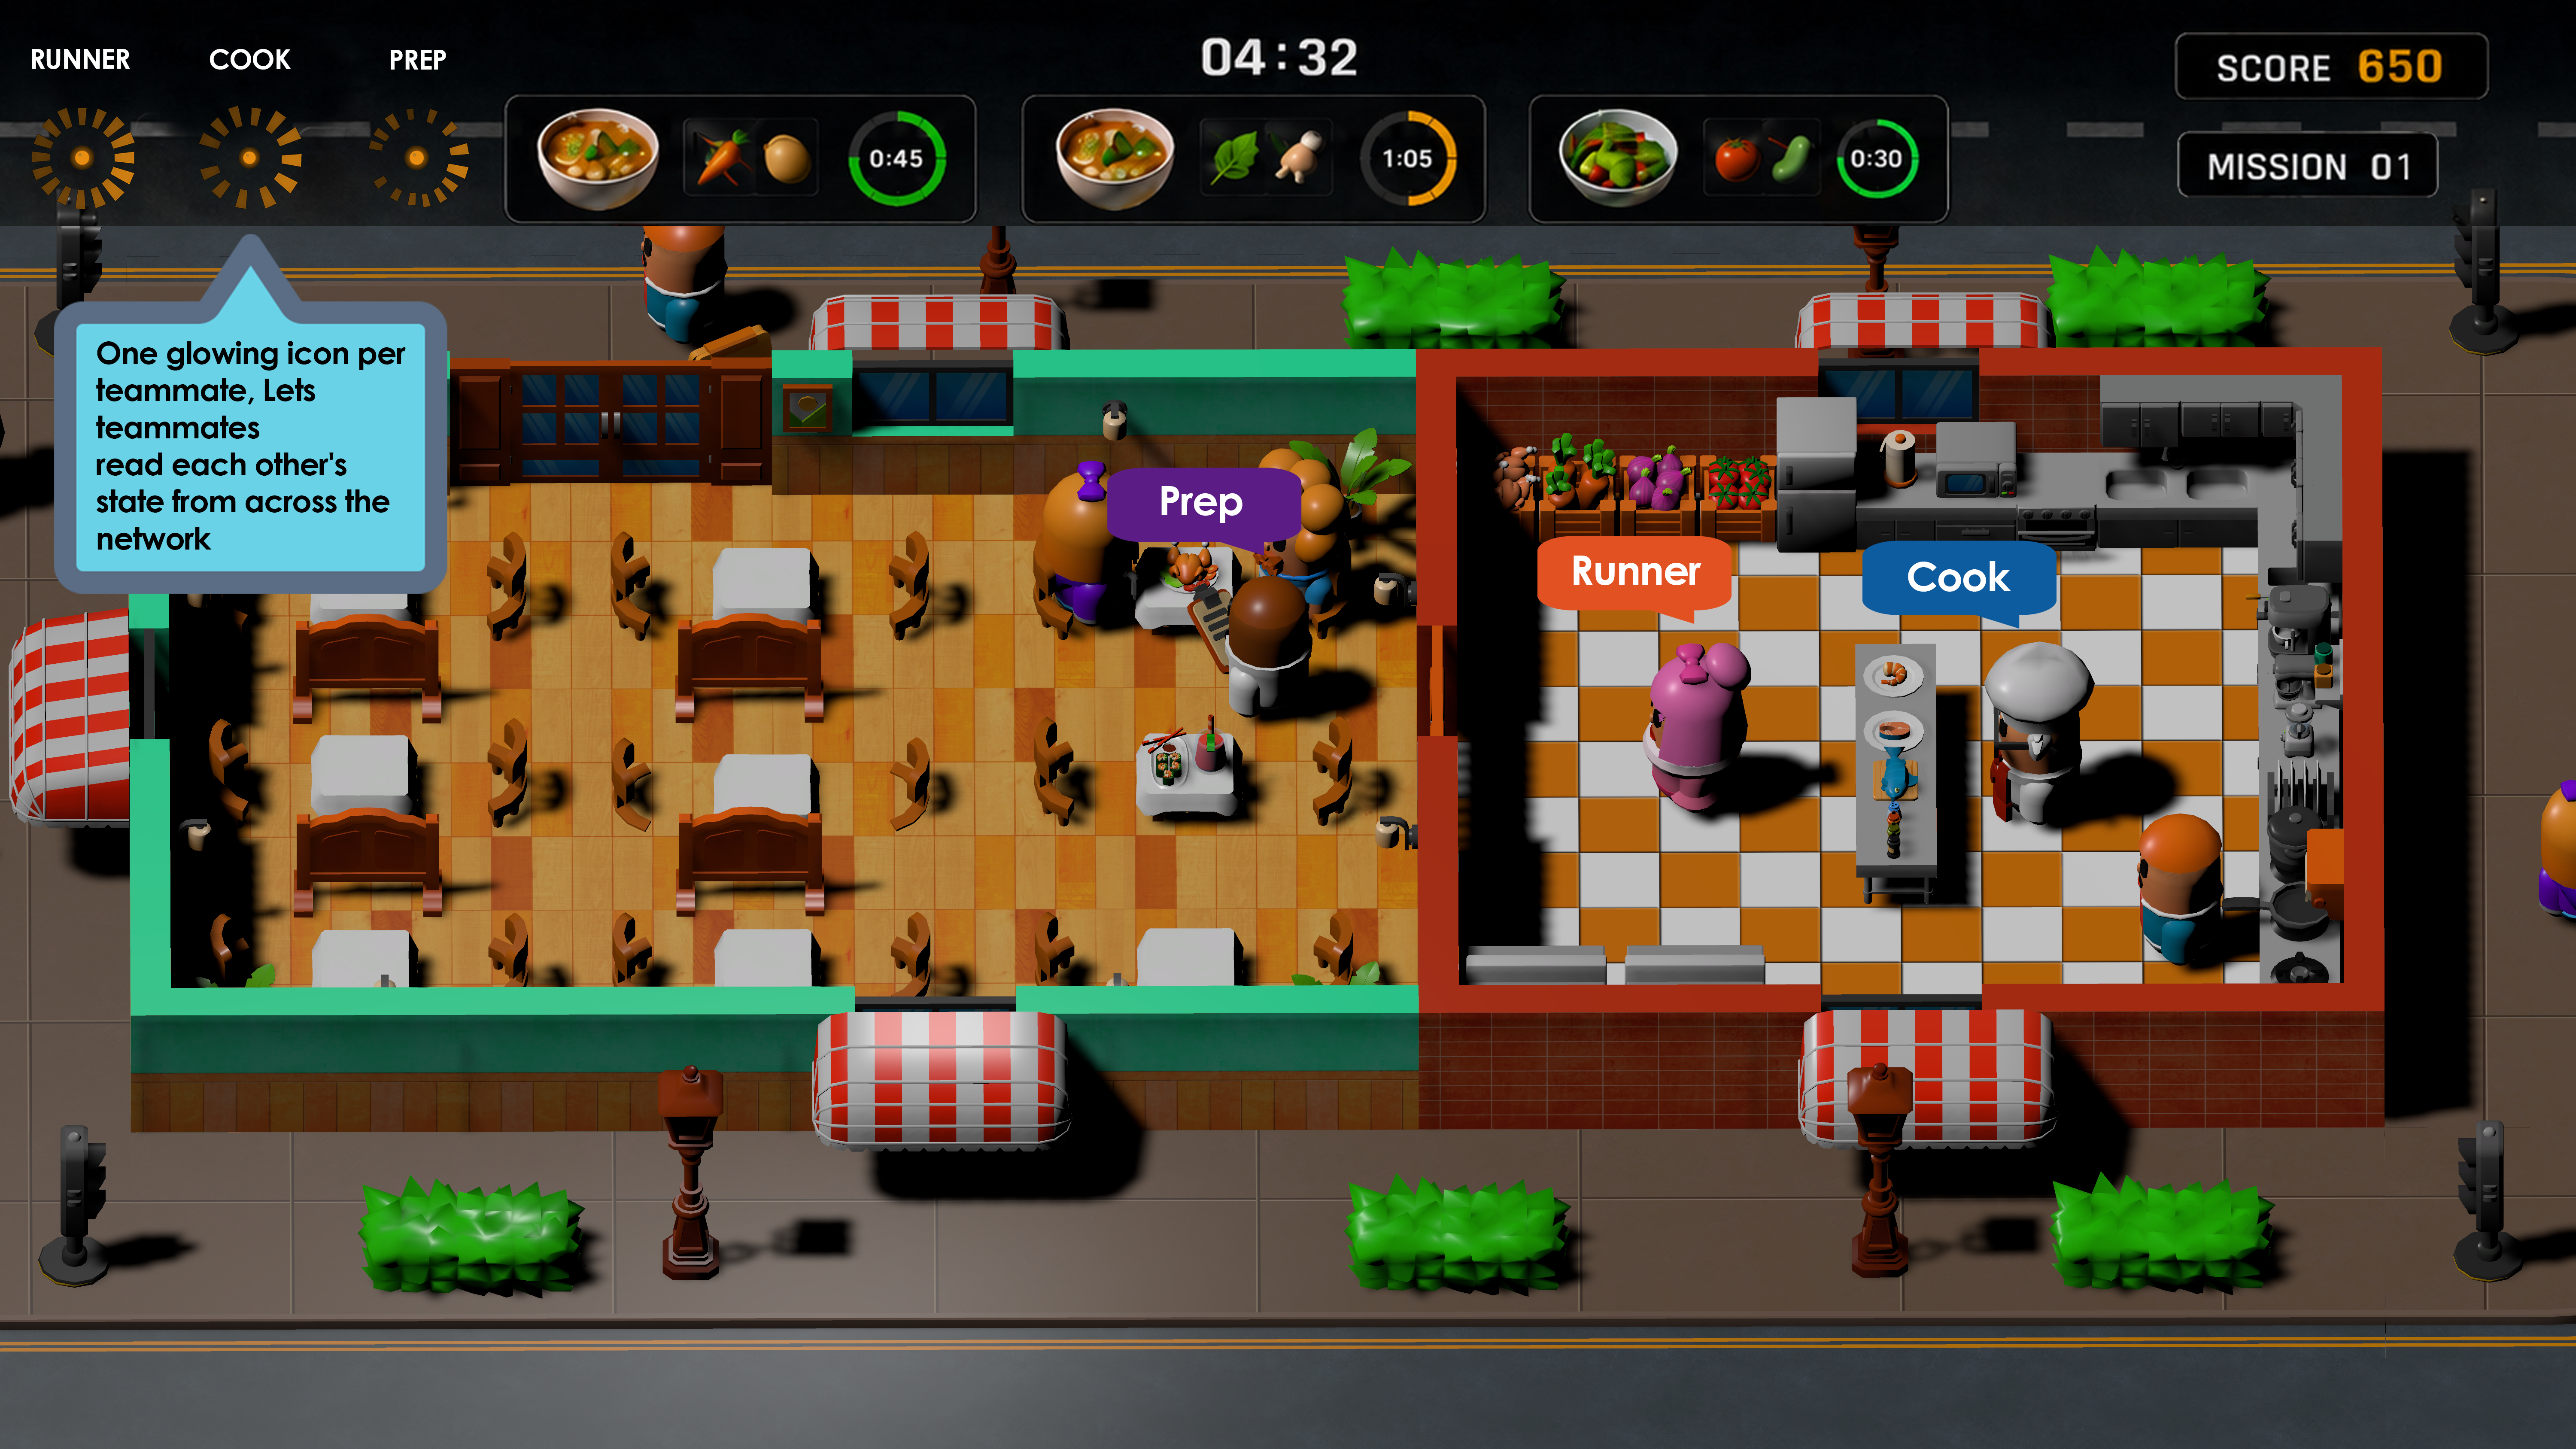
\includegraphics[width=0.82\textwidth]{Figure_1_Teaser_IconCue_Annotated.png}
  \caption{The Unity cooperative-cooking prototype with the Icon Cue. \rev{Each remote teammate has a physiological halo; HR sets its pulse and glow, and HRV the coherence of its ring. The physiological cue carries no numeric readout or emotion label.}}
  \Description{A top-down cooperative cooking game with a dining area and kitchen. A status bar shows three glowing circular icons labeled Runner, Cook, and Prep, with no numeric or text labels, and a callout: one glowing icon per teammate lets teammates read each other's state from across the network.}
  \label{fig:teaser}
\end{teaserfigure}

\maketitle

%% =====================================================================
\section{Introduction}
In a shared room, teammates register a partner's quickened breath and rising tension continuously and prereflectively. Distributed interaction removes much of this layer: remote partners infer effort from text, voice, and avatar motion, and removing face-to-face cues makes collaborators judge one another less accurately \cite{tan_role_2014}. Two recurring approaches in prior work are affective inference from sensed signals and explicit physiological sharing. Affective computing established a tradition of inferring affective states from sensed signals \cite{picard_affective_1997}, while physiological-sharing systems have explored how biosignals can support awareness and social connection \cite{hassib_heartchat_2017}. Howell et al.'s ambiguous skin-conductance display withholds fixed interpretive labels \cite{howell_biosignals_2016}; this work adds a separately encoded second channel and a chance-referenced legibility test.

We ask: \emph{can a remote teammate's physiological state remain readable, and useful for coordination, without converting the body into an explicit emotional or diagnostic label?} This work contributes to ISS at the intersection of body-worn sensing, peripheral displays, distributed interactive spaces, and group coordination. We contribute: (1) a design approach that translates Science and Technology Studies (STS) commitments into a compositional two-channel HR/HRV encoding; (2) chance-referenced evidence from Study~1 that the label-free representation is legible and graded; and (3) a live multiplayer evaluation showing that the Icon Cue accelerates teammate support relative to No Cue and \rev{shows no statistically significant difference from Numeric Cue on teammate awareness,} with lower workload and perceived invasiveness, while Numeric Cue \rev{remains higher on coordination usefulness and trust.}

%% =====================================================================
\section{Design: A Trace, Not a Verdict}
Classifications that persist and travel accumulate consequences for the people they sort \cite{bowker_sorting_2008}, measurement is not a neutral window onto a preexisting state \cite{barad_meeting_1996}, and any reading of a body is situated and partial \cite{haraway_situated_1988}. The display therefore offers a trace to interpret in context rather than a verdict to accept. Each teammate is one animated amber halo (Figure~\ref{fig:icons}). \textbf{Heart rate}, an index of momentary activation, controls pulse speed, glow, and expansion; \textbf{heart rate variability}, a marker of autonomic regulation \cite{thayer_model_2000}, controls ring coherence, from a smooth halo to a broken, jittering one. Each channel has four states relative to the player's own baseline, from HR1 (within $+5$\,bpm or 10\%) to HR4 (more than $+30$\,bpm or 45\% above), and from V1 ($\geq 110\%$ of baseline HRV) to V4 (below 60\%), giving 16 compositional states. These are prototype design states, not medical, clinical, or emotional diagnoses, and because they are baseline-relative they are not comparable across people. Hue stays a warm amber rather than an alarm red, and every state carries a small ambient shimmer so that the calmest state does not read as a flawless signal.

\begin{figure}[t]
  \centering
  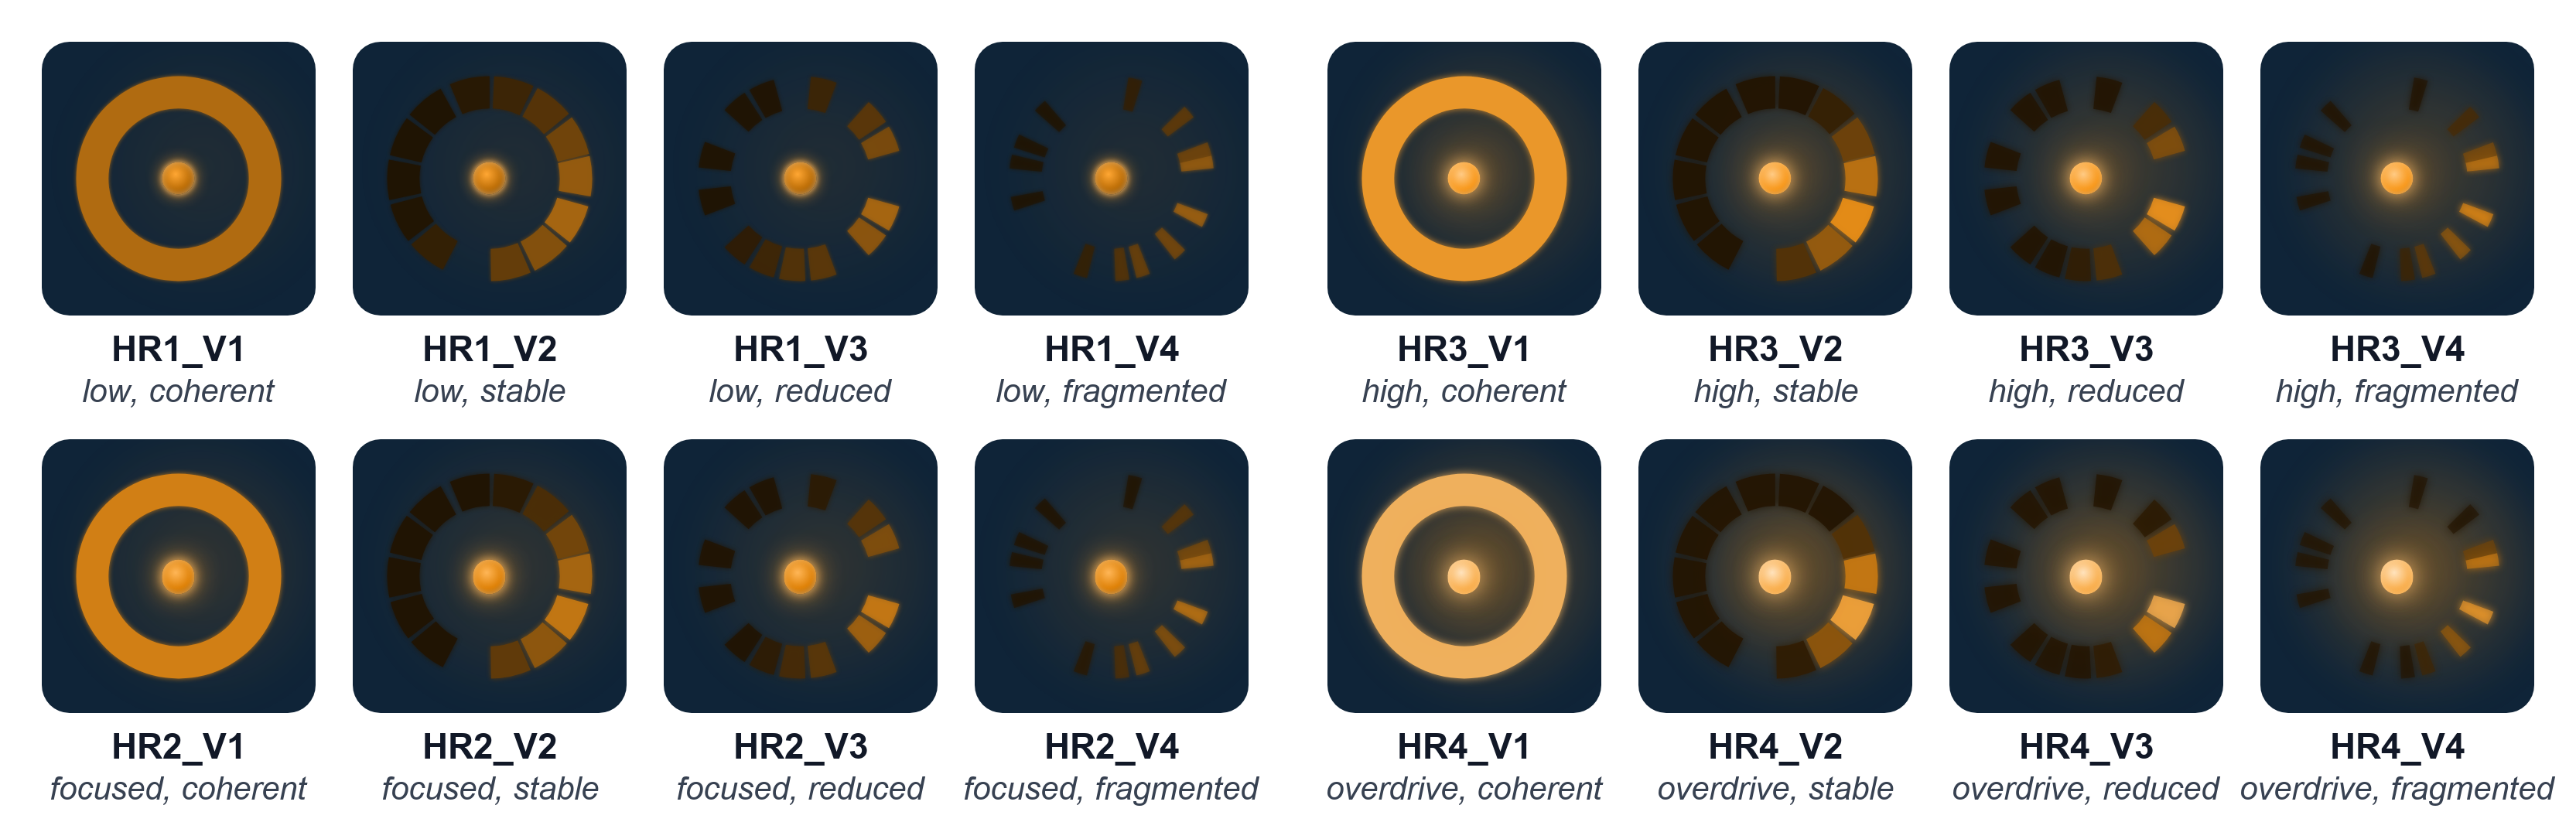
\includegraphics[width=\columnwidth]{Figure_Icon_Stimulus_Set_16_Conditions.png}
  \caption{The 16 halo states (HR1--HR4 $\times$ V1--V4). Brightness, bloom, and pulse speed encode HR; ring segmentation, jitter, and dropout encode HRV. Single frames of looping animations.}
  \Description{Sixteen circular status icons on dark tiles. Core brightness increases from HR1 to HR4, and ring segmentation becomes sparser and more irregular from V1 to V4.}
  \label{fig:icons}
\end{figure}

%% =====================================================================
\section{Study 1: Is the Halo Legible?}
Thirty-six adults took part online in a within-subjects study (Figure~\ref{fig:design}). In an open phase, they described four unlabeled states. In a structured phase, they viewed all 16 states in random order, identified the HR and HRV state from four options each, rated clarity, urgency, stability, coordination usefulness, and support intention, and completed the Self-Assessment Manikin (SAM) \cite{bradley_measuring_1994}; three NASA-TLX items \cite{hart_development_1988} closed the session. \rev{This is a recognition task: viewers judged isolated halo stimuli whose intended states were known.}

\rev{\textbf{Analysis.}} Following the ISO~9186 convention \cite{iso_9186_2014}, \rev{participant-level accuracy was compared with chance using two-sided one-sample $t$ tests, with Cohen's $d_z$. All four pre-specified legibility comparisons also survived a conservative Bonferroni threshold of $\alpha=.0125$. Planned linear trends were Holm-corrected across five tests. Free-text interpretations and open responses were analyzed using reflexive thematic analysis \revcite{braun_using_2006}.}

\begin{figure*}[t]
  \centering
  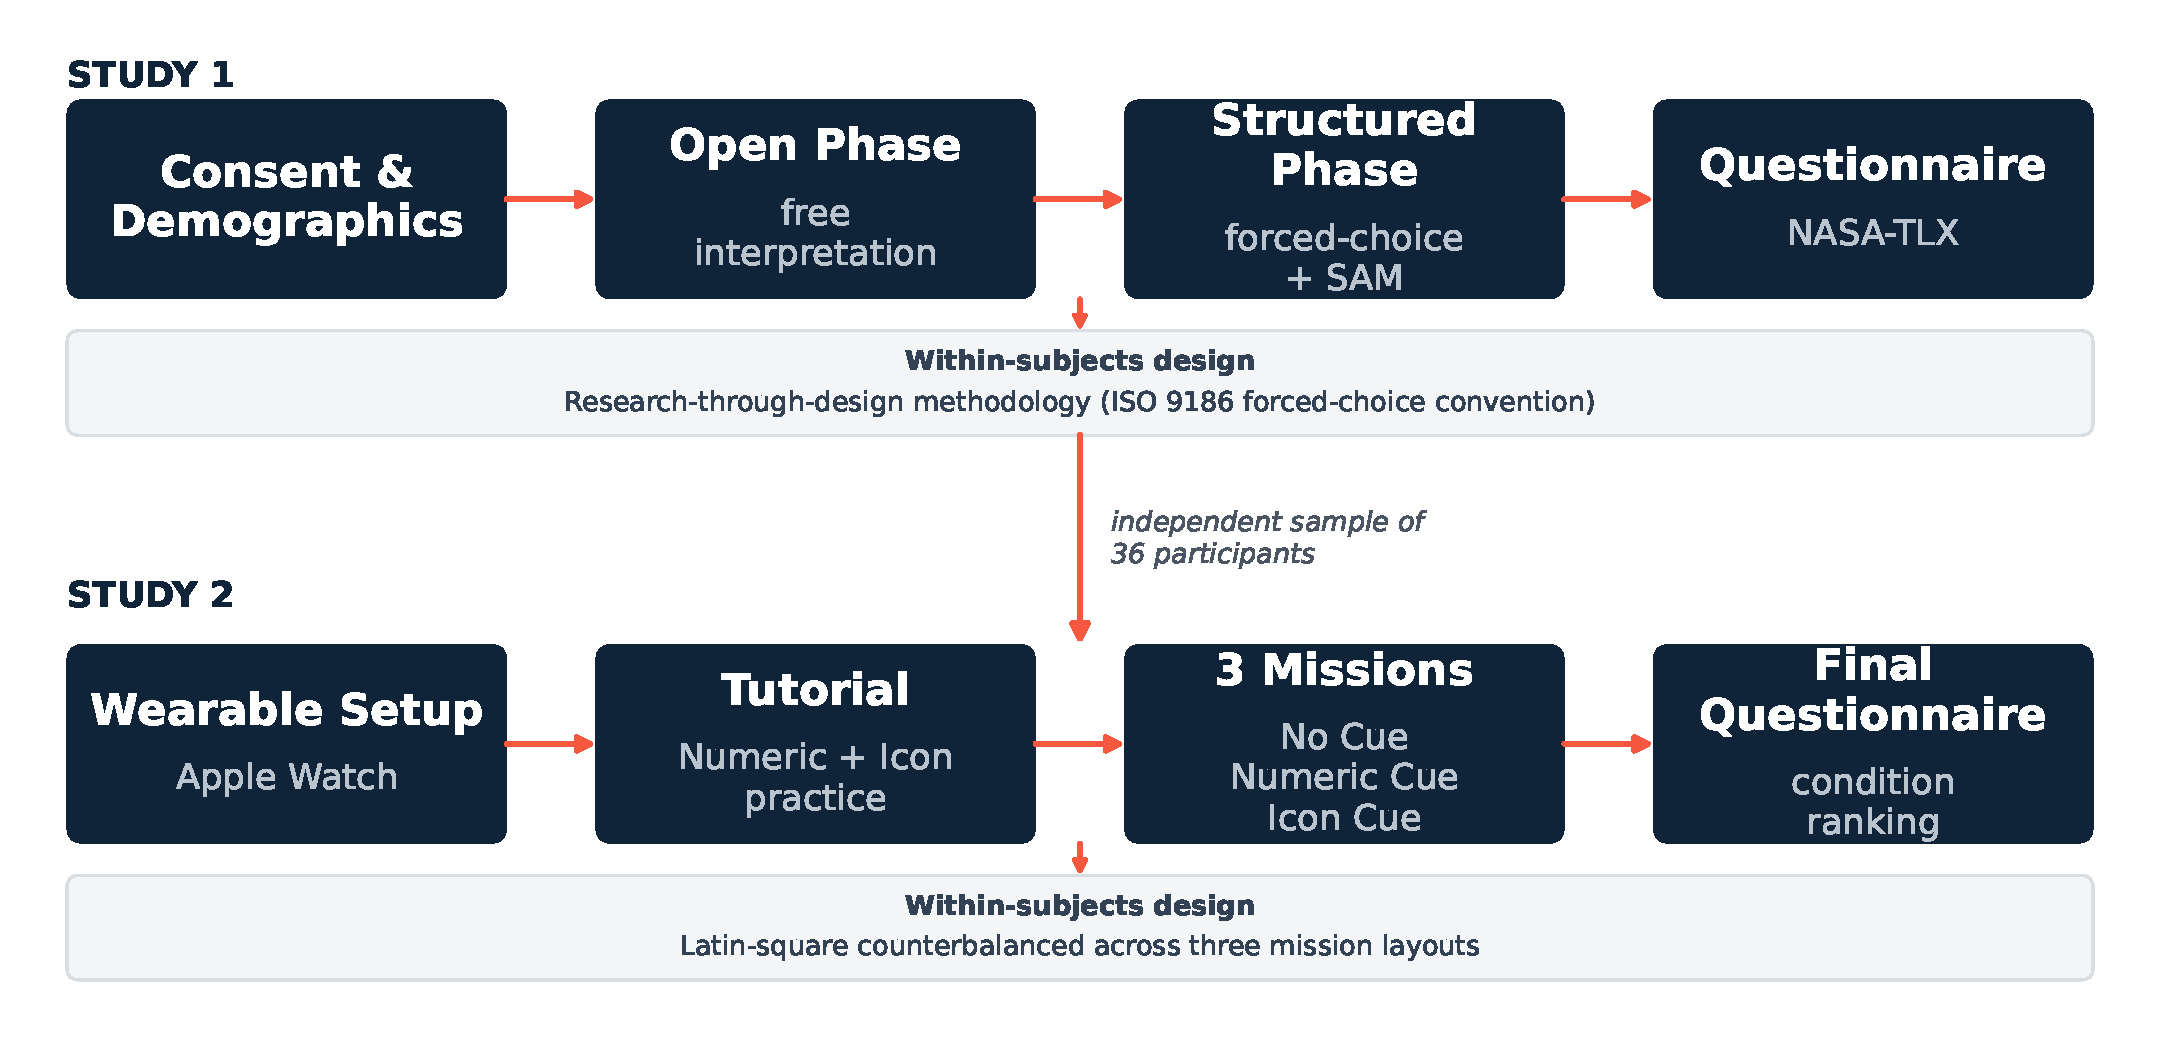
\includegraphics[width=0.62\textwidth]{Figure_Study_Design_Walkthrough.pdf}
  \caption{Study design. Study~1: online legibility study. Study~2: independent sample of three-player teams across three counterbalanced conditions.}
  \Description{A two-row flow diagram. Study 1: consent, open phase, structured forced-choice phase with SAM, NASA-TLX questionnaire. Study 2: wearable setup and baseline, matched tutorial, three missions (No Cue, Numeric Cue, Icon Cue), and a final ranking questionnaire.}
  \label{fig:design}
\end{figure*}

\rev{\textbf{Results.}} Participants identified the HR state on \textbf{66.3\%} of trials (95\% CI 58.5--74.2) and the HRV state on \textbf{58.2\%} (95\% CI 51.0--65.3), both above 25\% chance ($p<.001$). Joint identification reached \textbf{44.6\%} against 6.25\% chance ($t(35)=9.90$, $p<.001$), and the hardest joint cell reached 33.3\%, more than five times chance (Figure~\ref{fig:s1}). Holm-corrected linear trends showed that higher HR raised perceived urgency and arousal, and that a more fragmented ring lowered perceived stability and raised support intention by \textbf{0.48 points per HRV level} ($t(35)=7.78$, $p<.001$). Clarity averaged 5.22/7 and coordination usefulness 5.45/7; mental demand (3.64), effort (3.47), and frustration (2.53) remained below the scale midpoint.

\begin{figure*}[t]
  \centering
  \begin{subfigure}[b]{0.34\textwidth}
    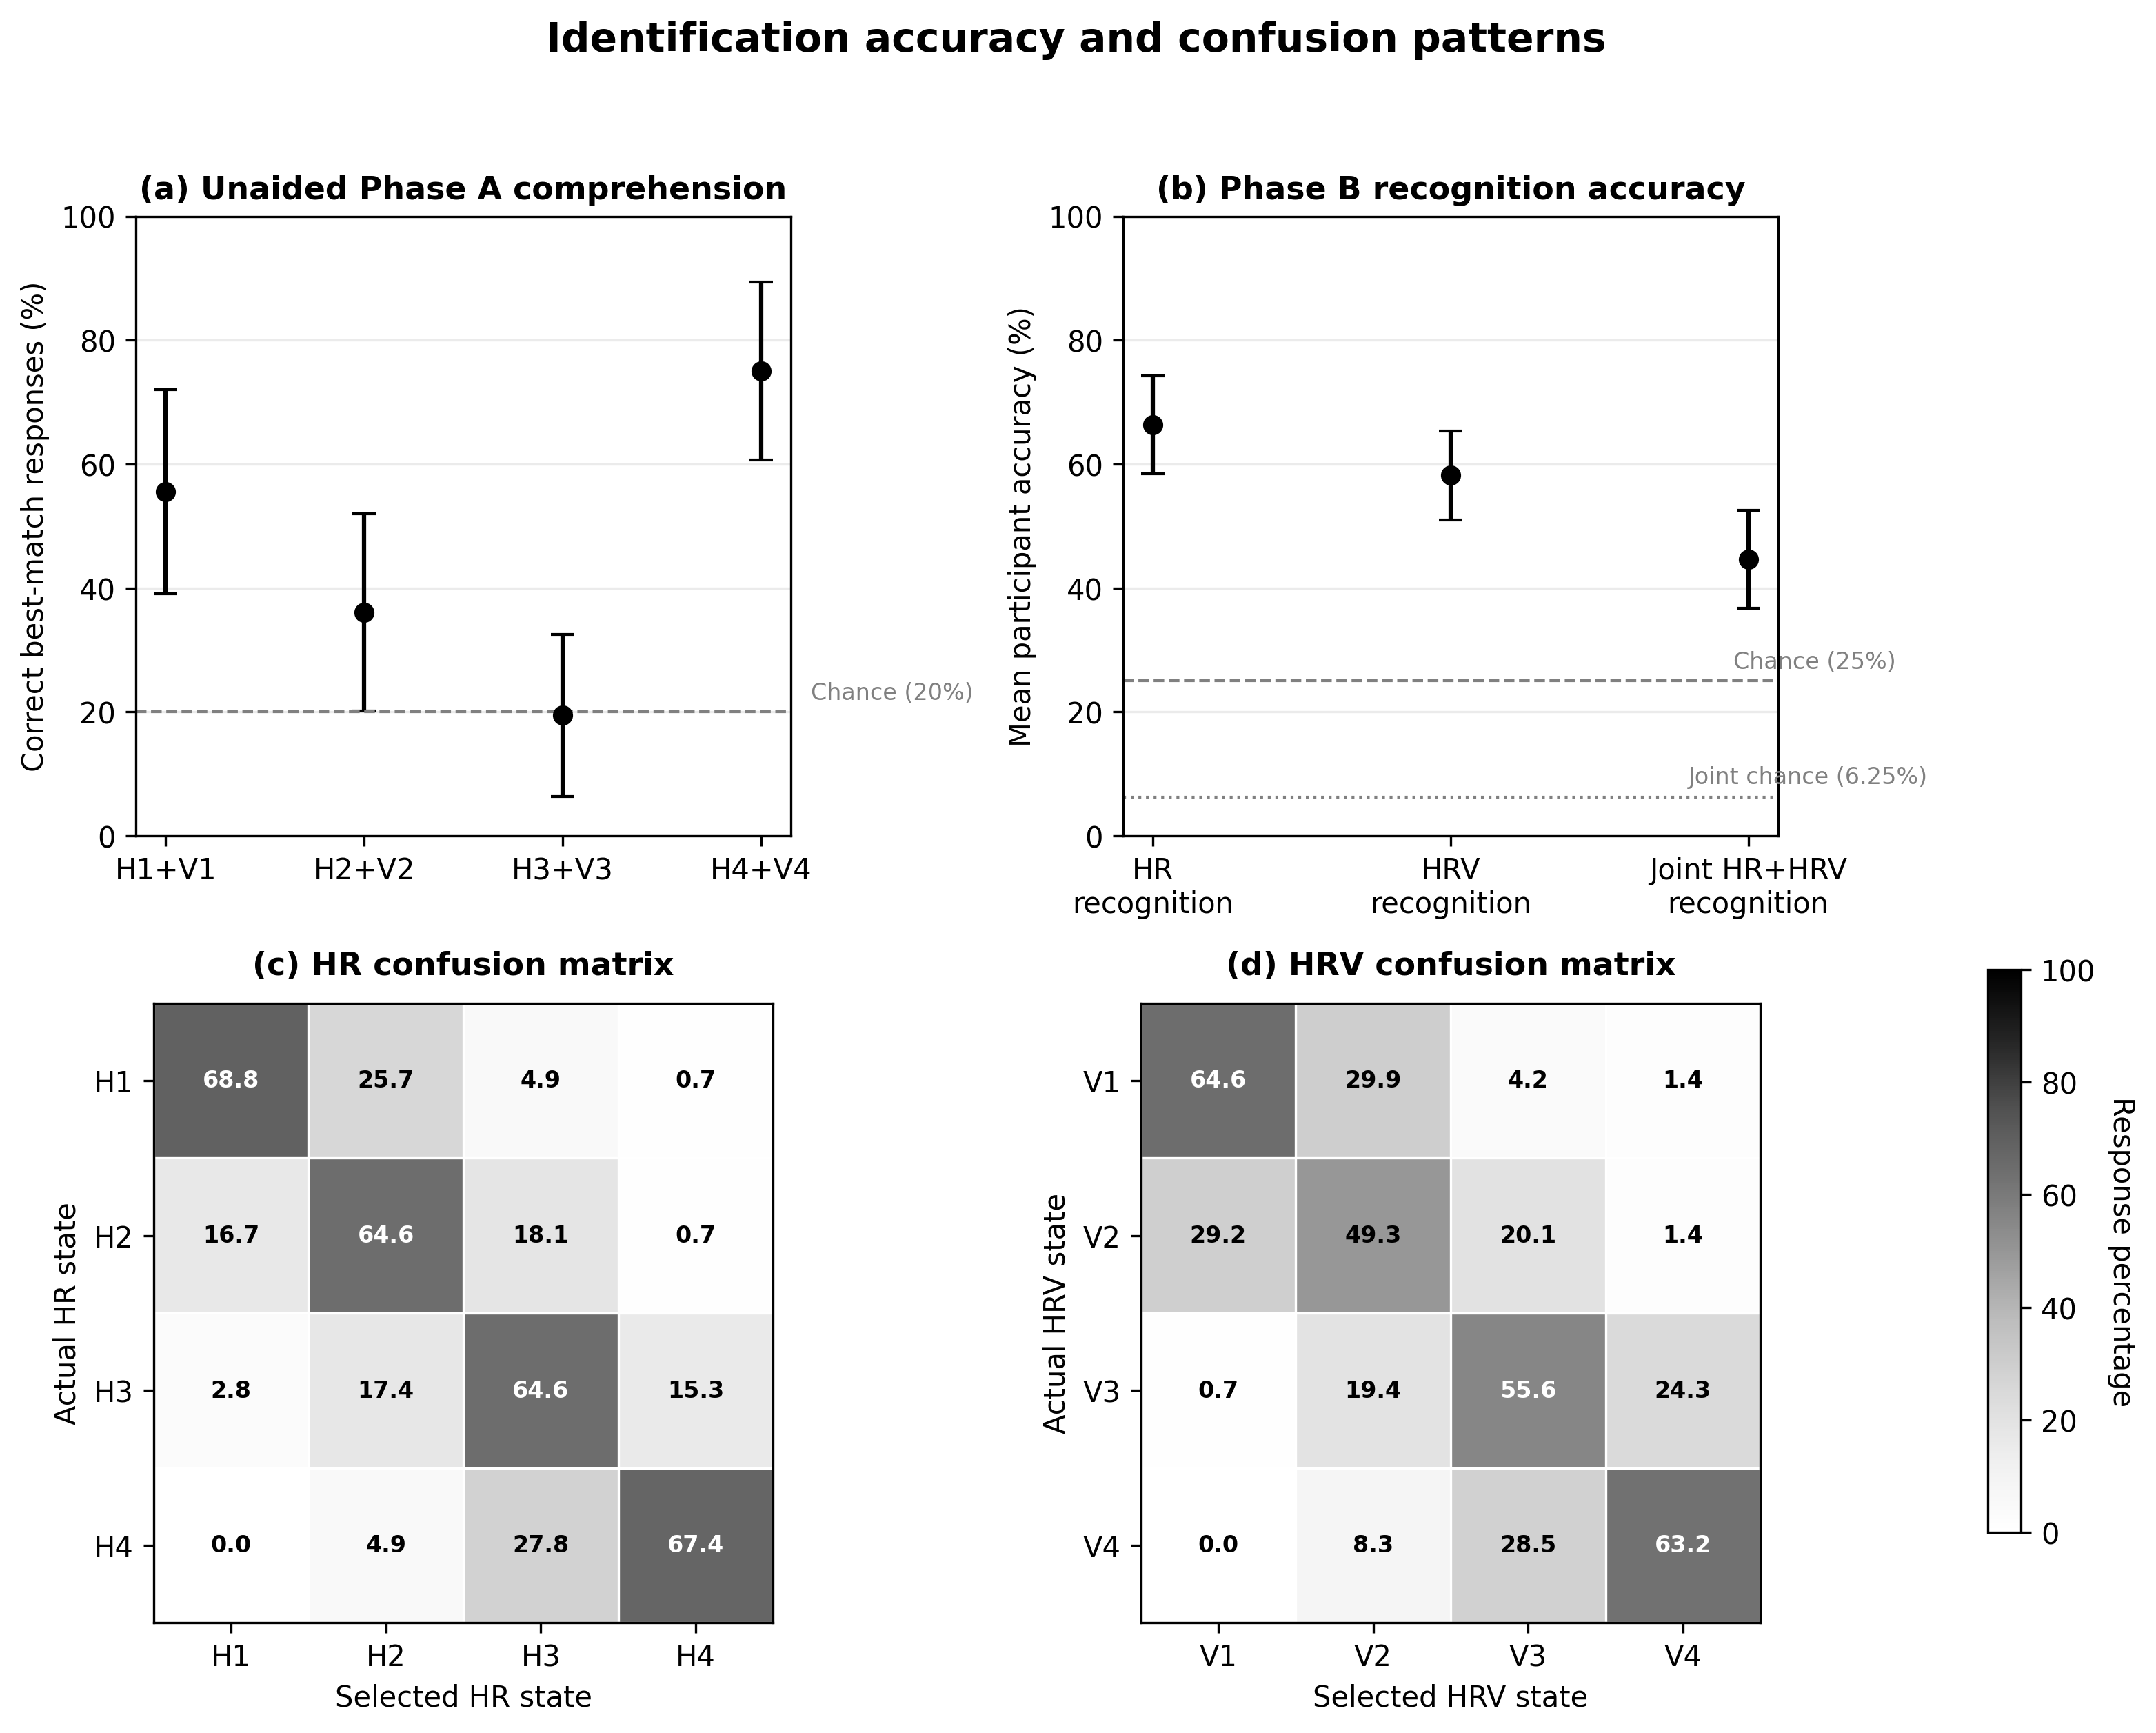
\includegraphics[width=\linewidth]{Figure_4_Identification_Accuracy_Confusion.png}
    \caption{Recognition accuracy and confusion matrices.}
  \end{subfigure}\hfill
  \begin{subfigure}[b]{0.62\textwidth}
    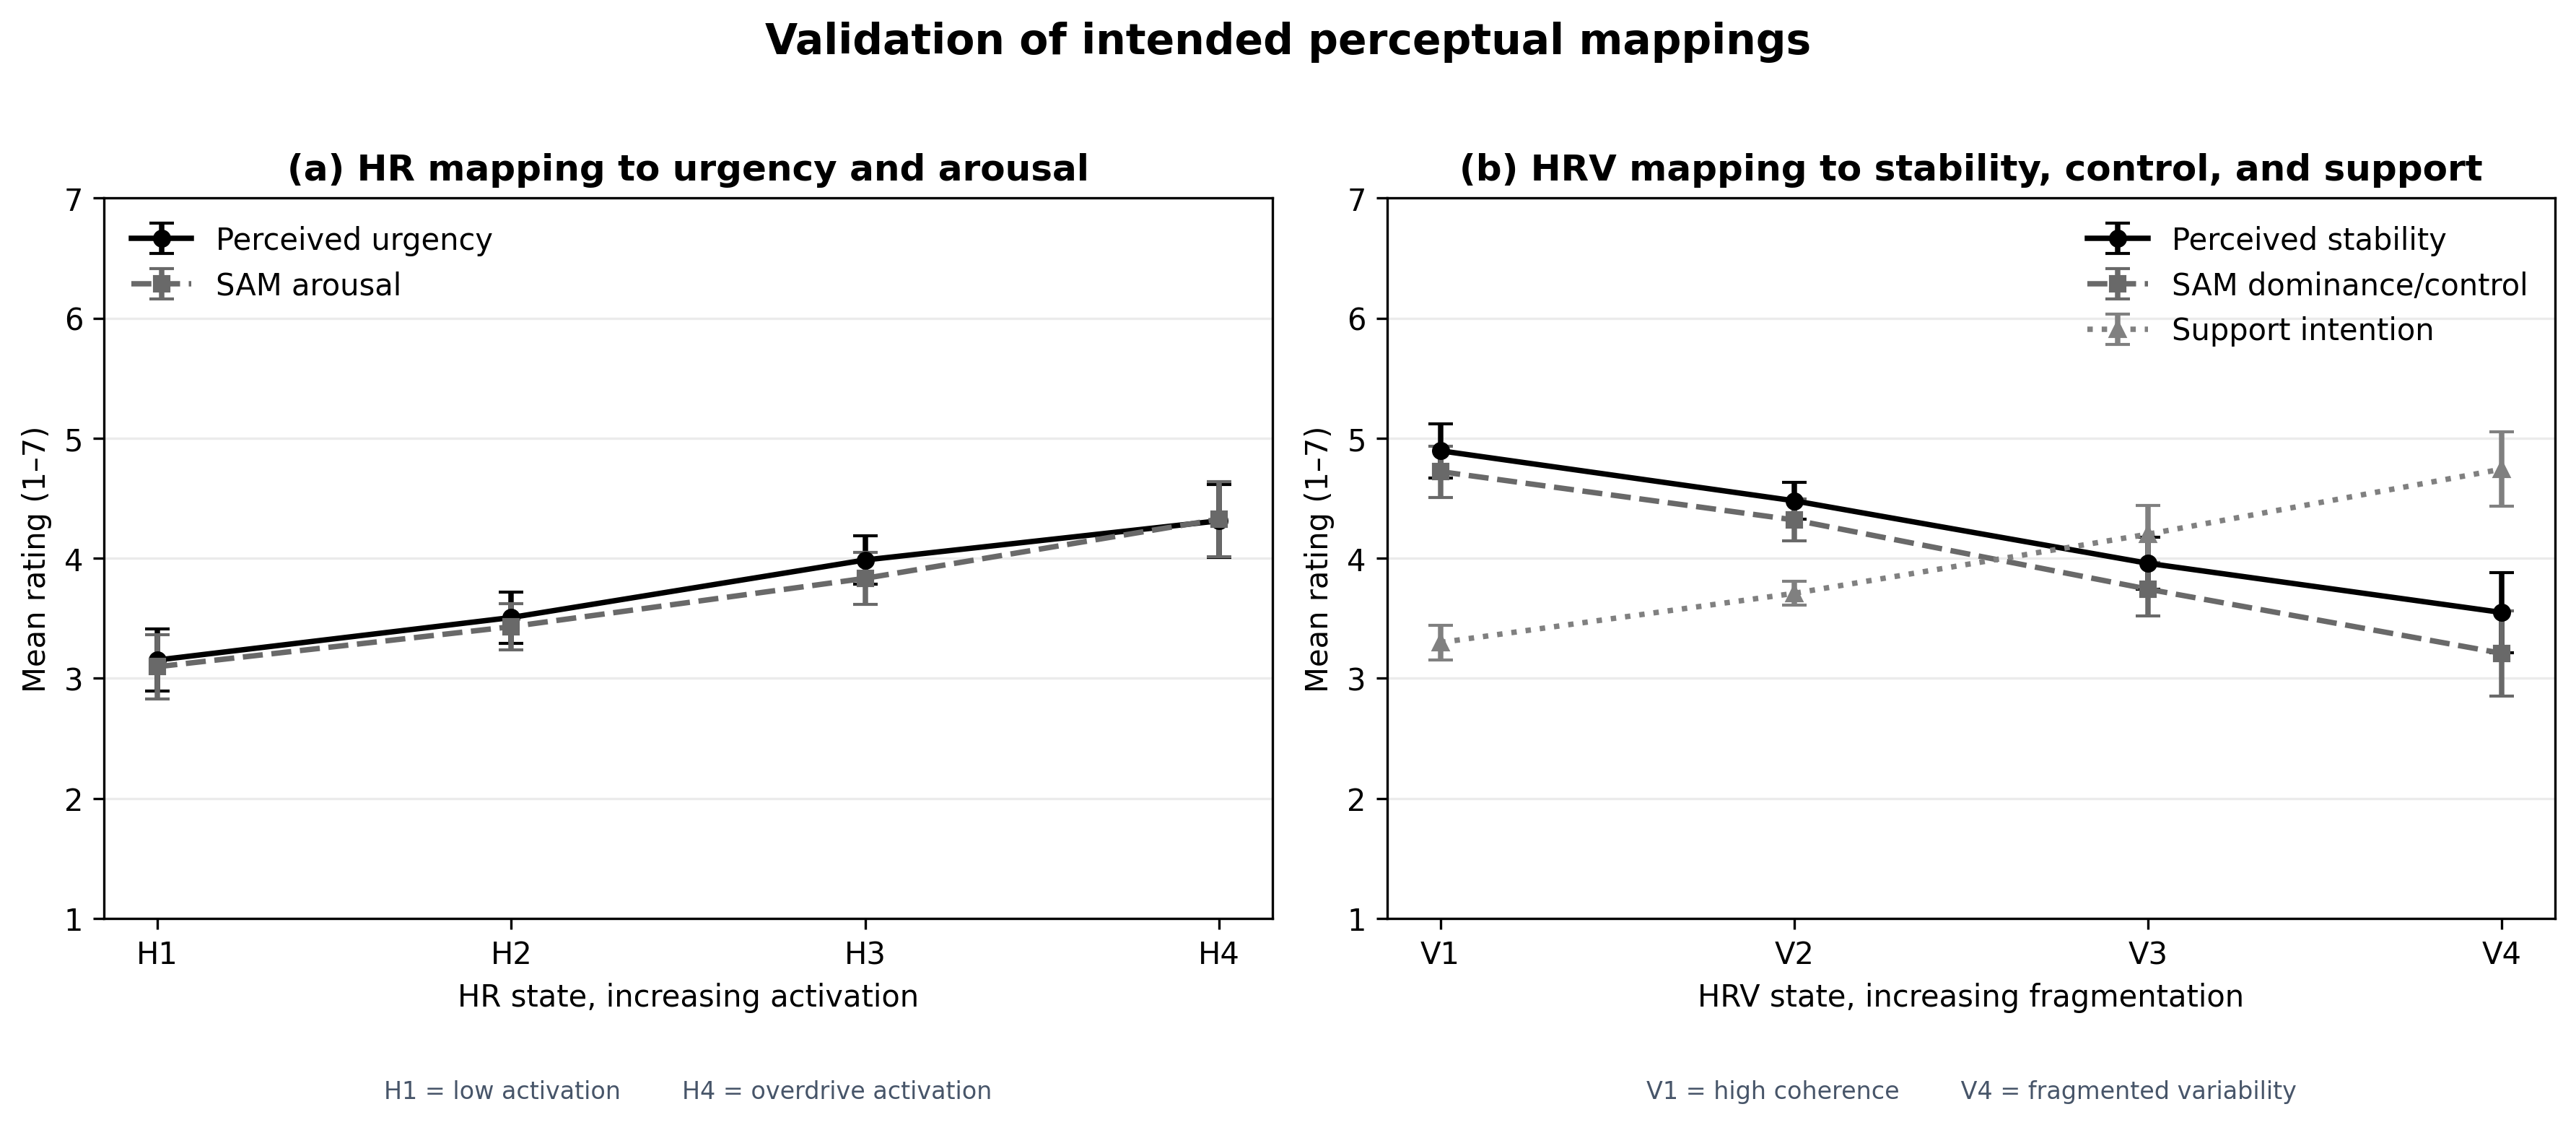
\includegraphics[width=\linewidth]{Figure_5_Perceptual_Mappings.png}
    \caption{Perceptual mappings for HR and HRV.}
  \end{subfigure}
  \caption{Study~1 results. Error bars show 95\% confidence intervals.}
  \Description{Two panels: recognition accuracy against chance with HR and HRV confusion matrices; and line charts of urgency and arousal across HR states, and of stability, control, and support intention across HRV states.}
  \label{fig:s1}
\end{figure*}

%% =====================================================================
\section{Study 2: Live Multiplayer Evaluation}
\textbf{Method.} An independent sample of 36 participants formed 12 teams of three (Prep, Cook, Runner) and played a custom Unity cooperative-cooking task modeled on Overcooked \cite{carroll_utility_2019} from separate locations (Figure~\ref{fig:s2setup}). Each player wore an Apple Watch; a HealthKit companion app exposed HR and beat-to-beat data, and a local bridge classified each player's HR and RMSSD-based HRV state against a three-minute seated baseline \cite{lopes_architecture_2023}. Only the resulting classified HR/HRV state values were replicated to remote clients; raw physiological time series remained local. Each team played three seven-minute missions, one per condition (\textbf{No Cue}; \textbf{Numeric Cue}, HR in bpm and HRV in ms; \textbf{Icon Cue}, the halo), Latin-square counterbalanced after a matched tutorial. \rev{Each mission included three researcher-triggered task events: \emph{Ingredient Bottleneck} near 2:00, when two orders required the same ingredient; \emph{Pot Overload} near 4:30, when two pots became active close together; and \emph{Service Rush} in the final phase, when completed dishes, dirty plates, and delivery tasks accumulated. These events targeted Prep, Cook, and Runner, respectively. Physiological input remained live; the task events were scripted.} Questionnaires followed each condition.

\begin{figure*}[t]
  \centering
  \begin{subfigure}[b]{0.192\textwidth}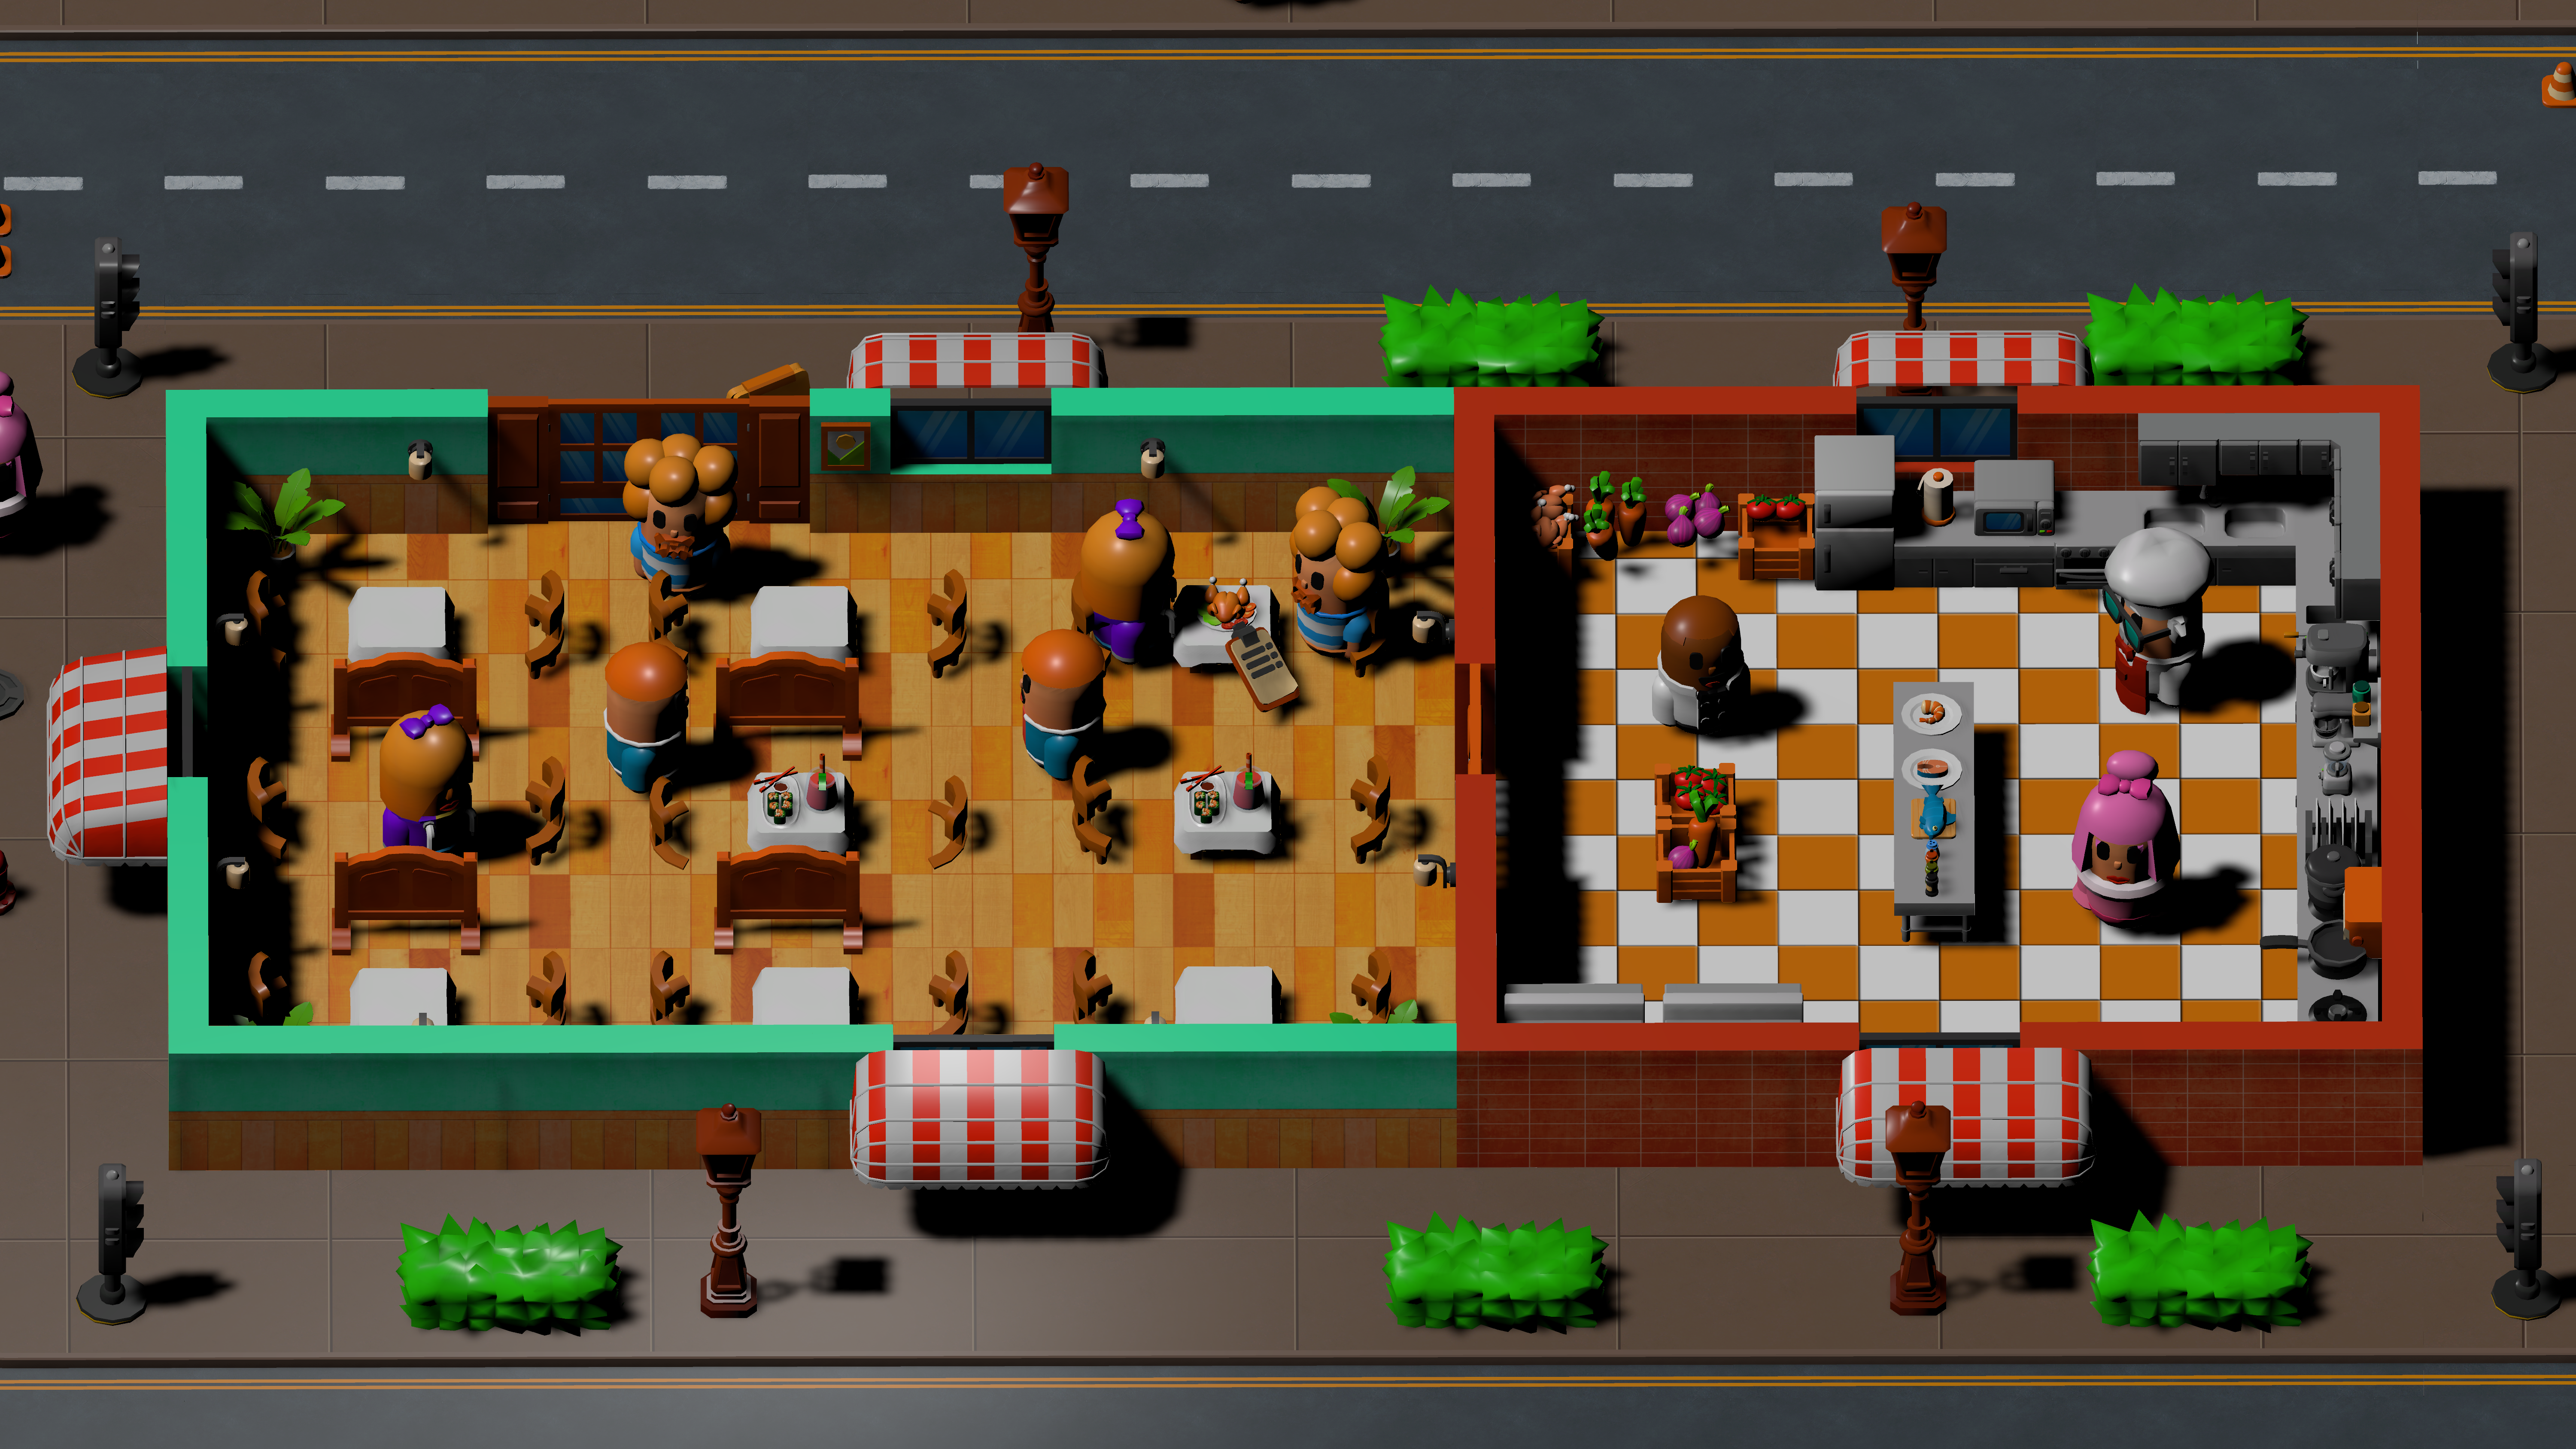
\includegraphics[width=\linewidth]{Figure_Environment_Overview.png}\caption{Environment}\end{subfigure}\hfill
  \begin{subfigure}[b]{0.192\textwidth}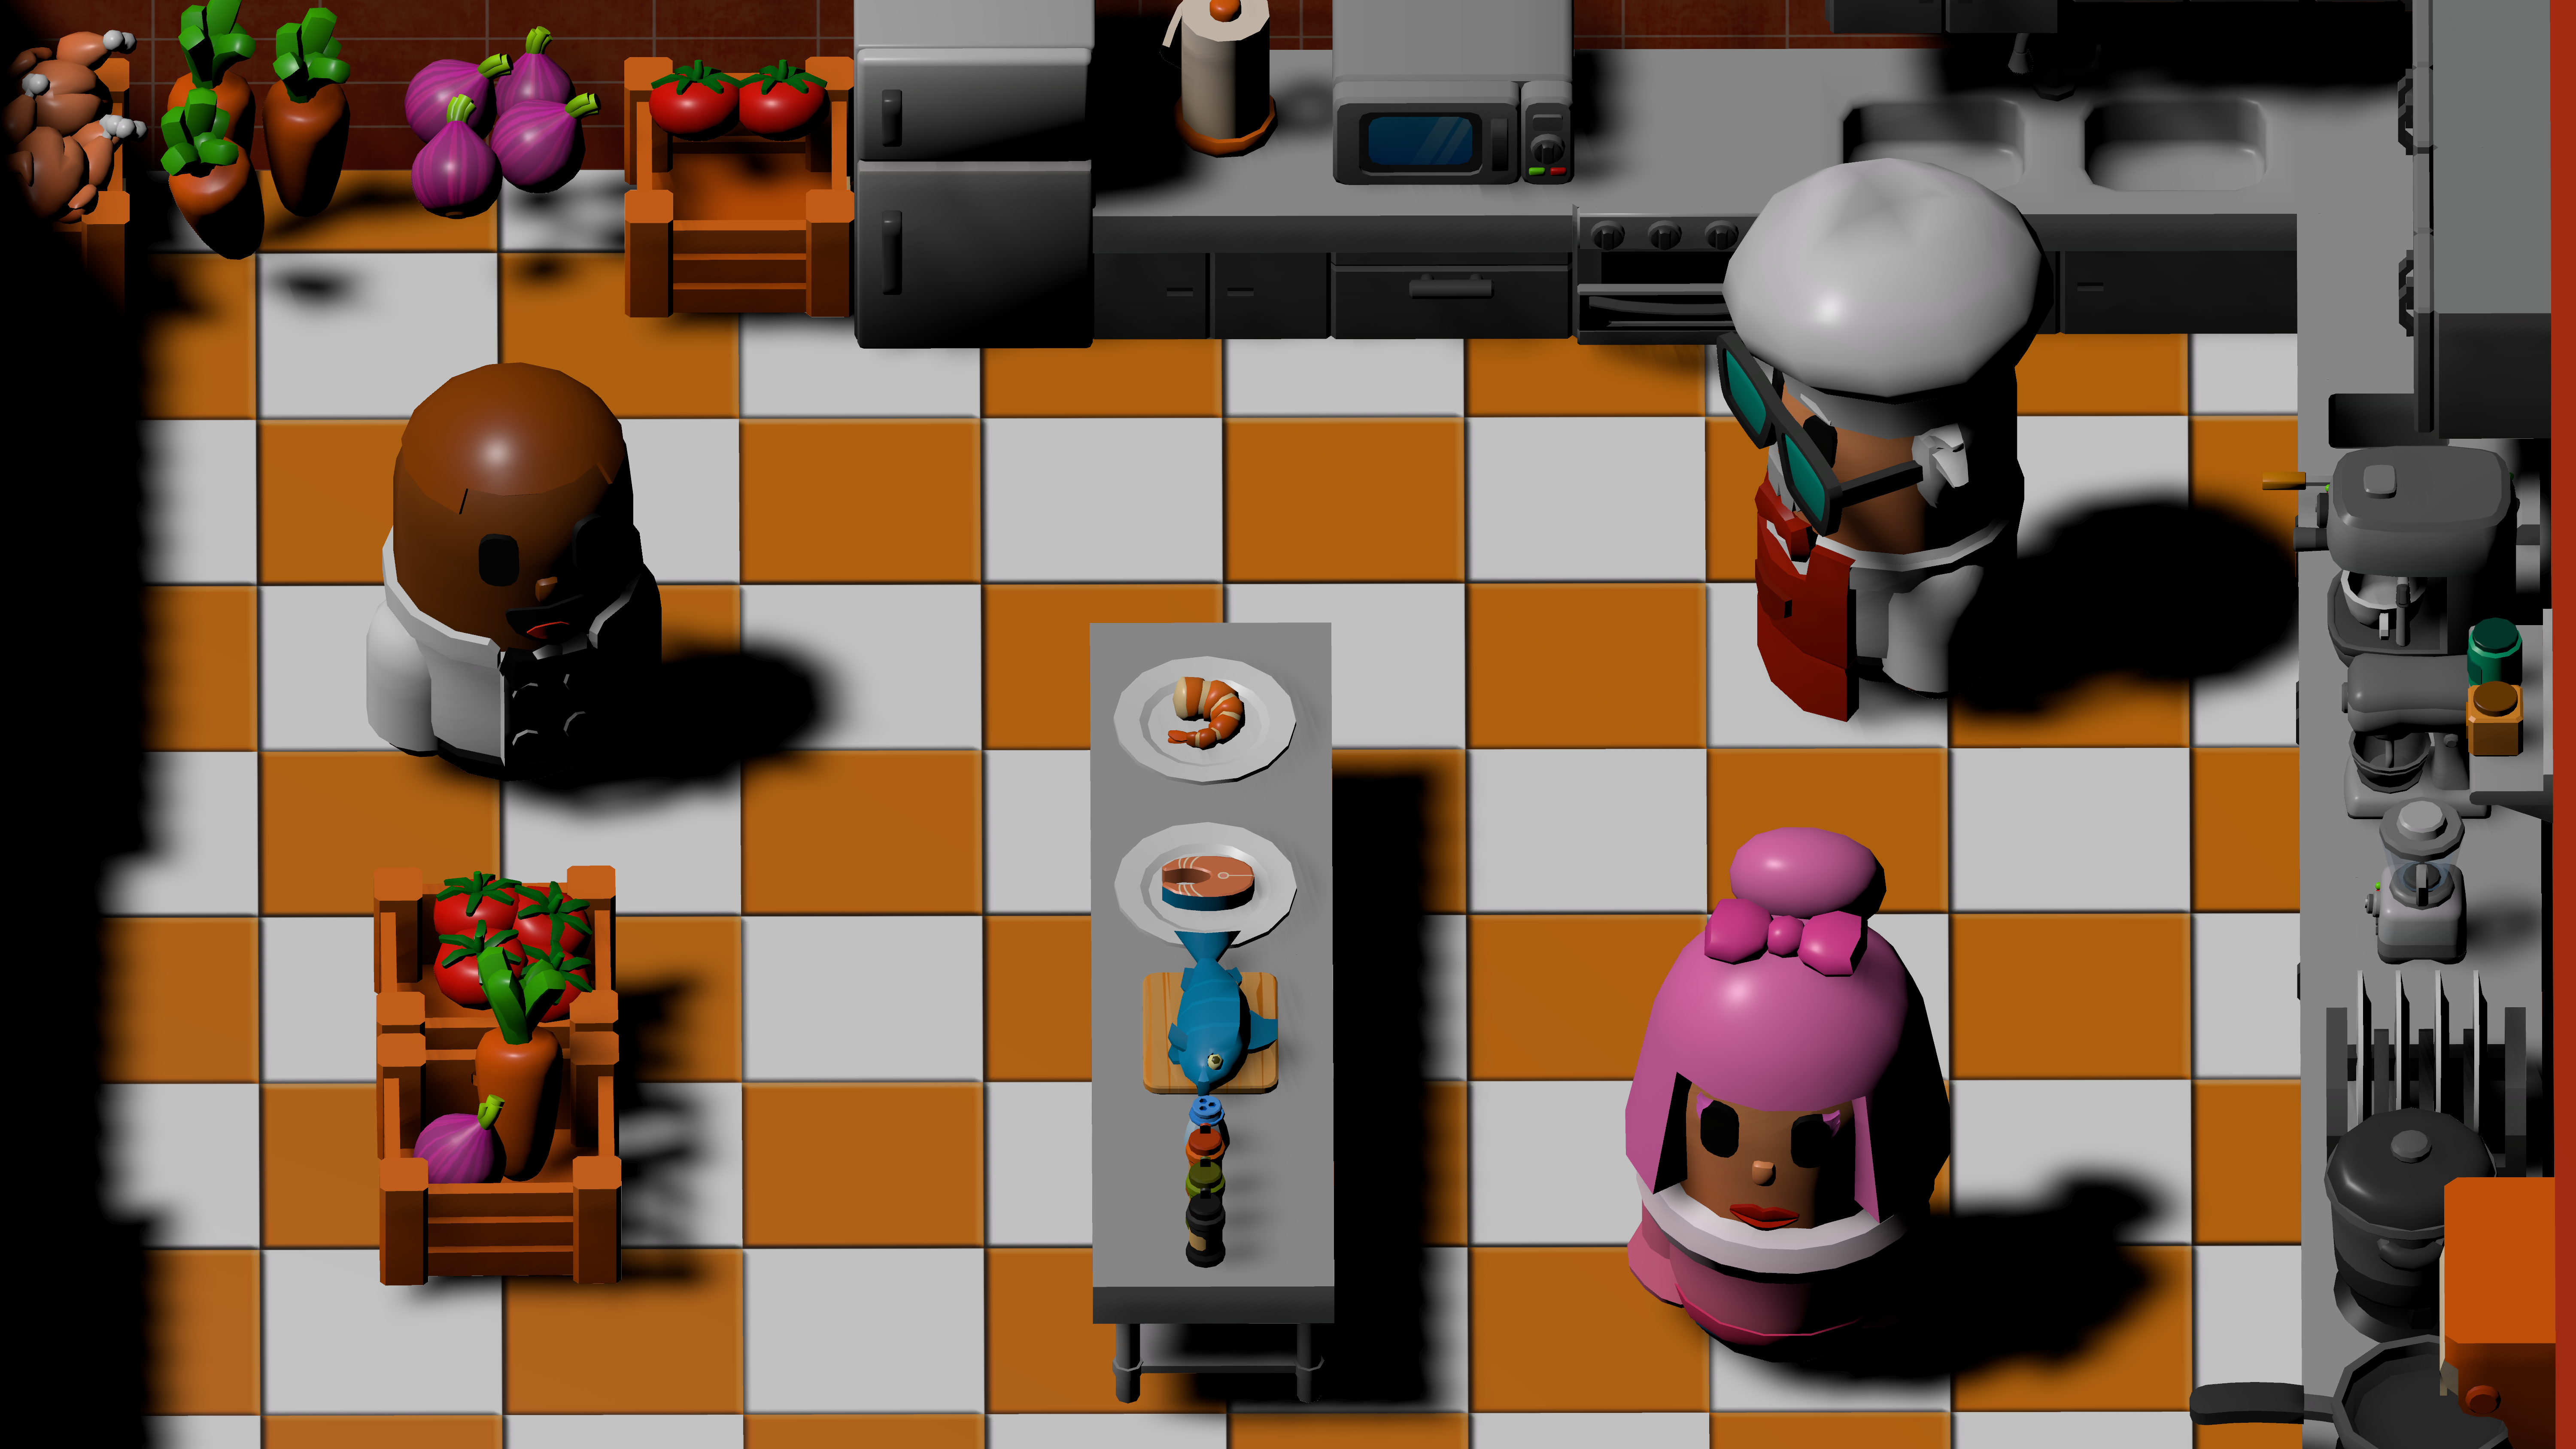
\includegraphics[width=\linewidth]{Figure_Environment_Kitchen_Detail.png}\caption{Kitchen}\end{subfigure}\hfill
  \begin{subfigure}[b]{0.192\textwidth}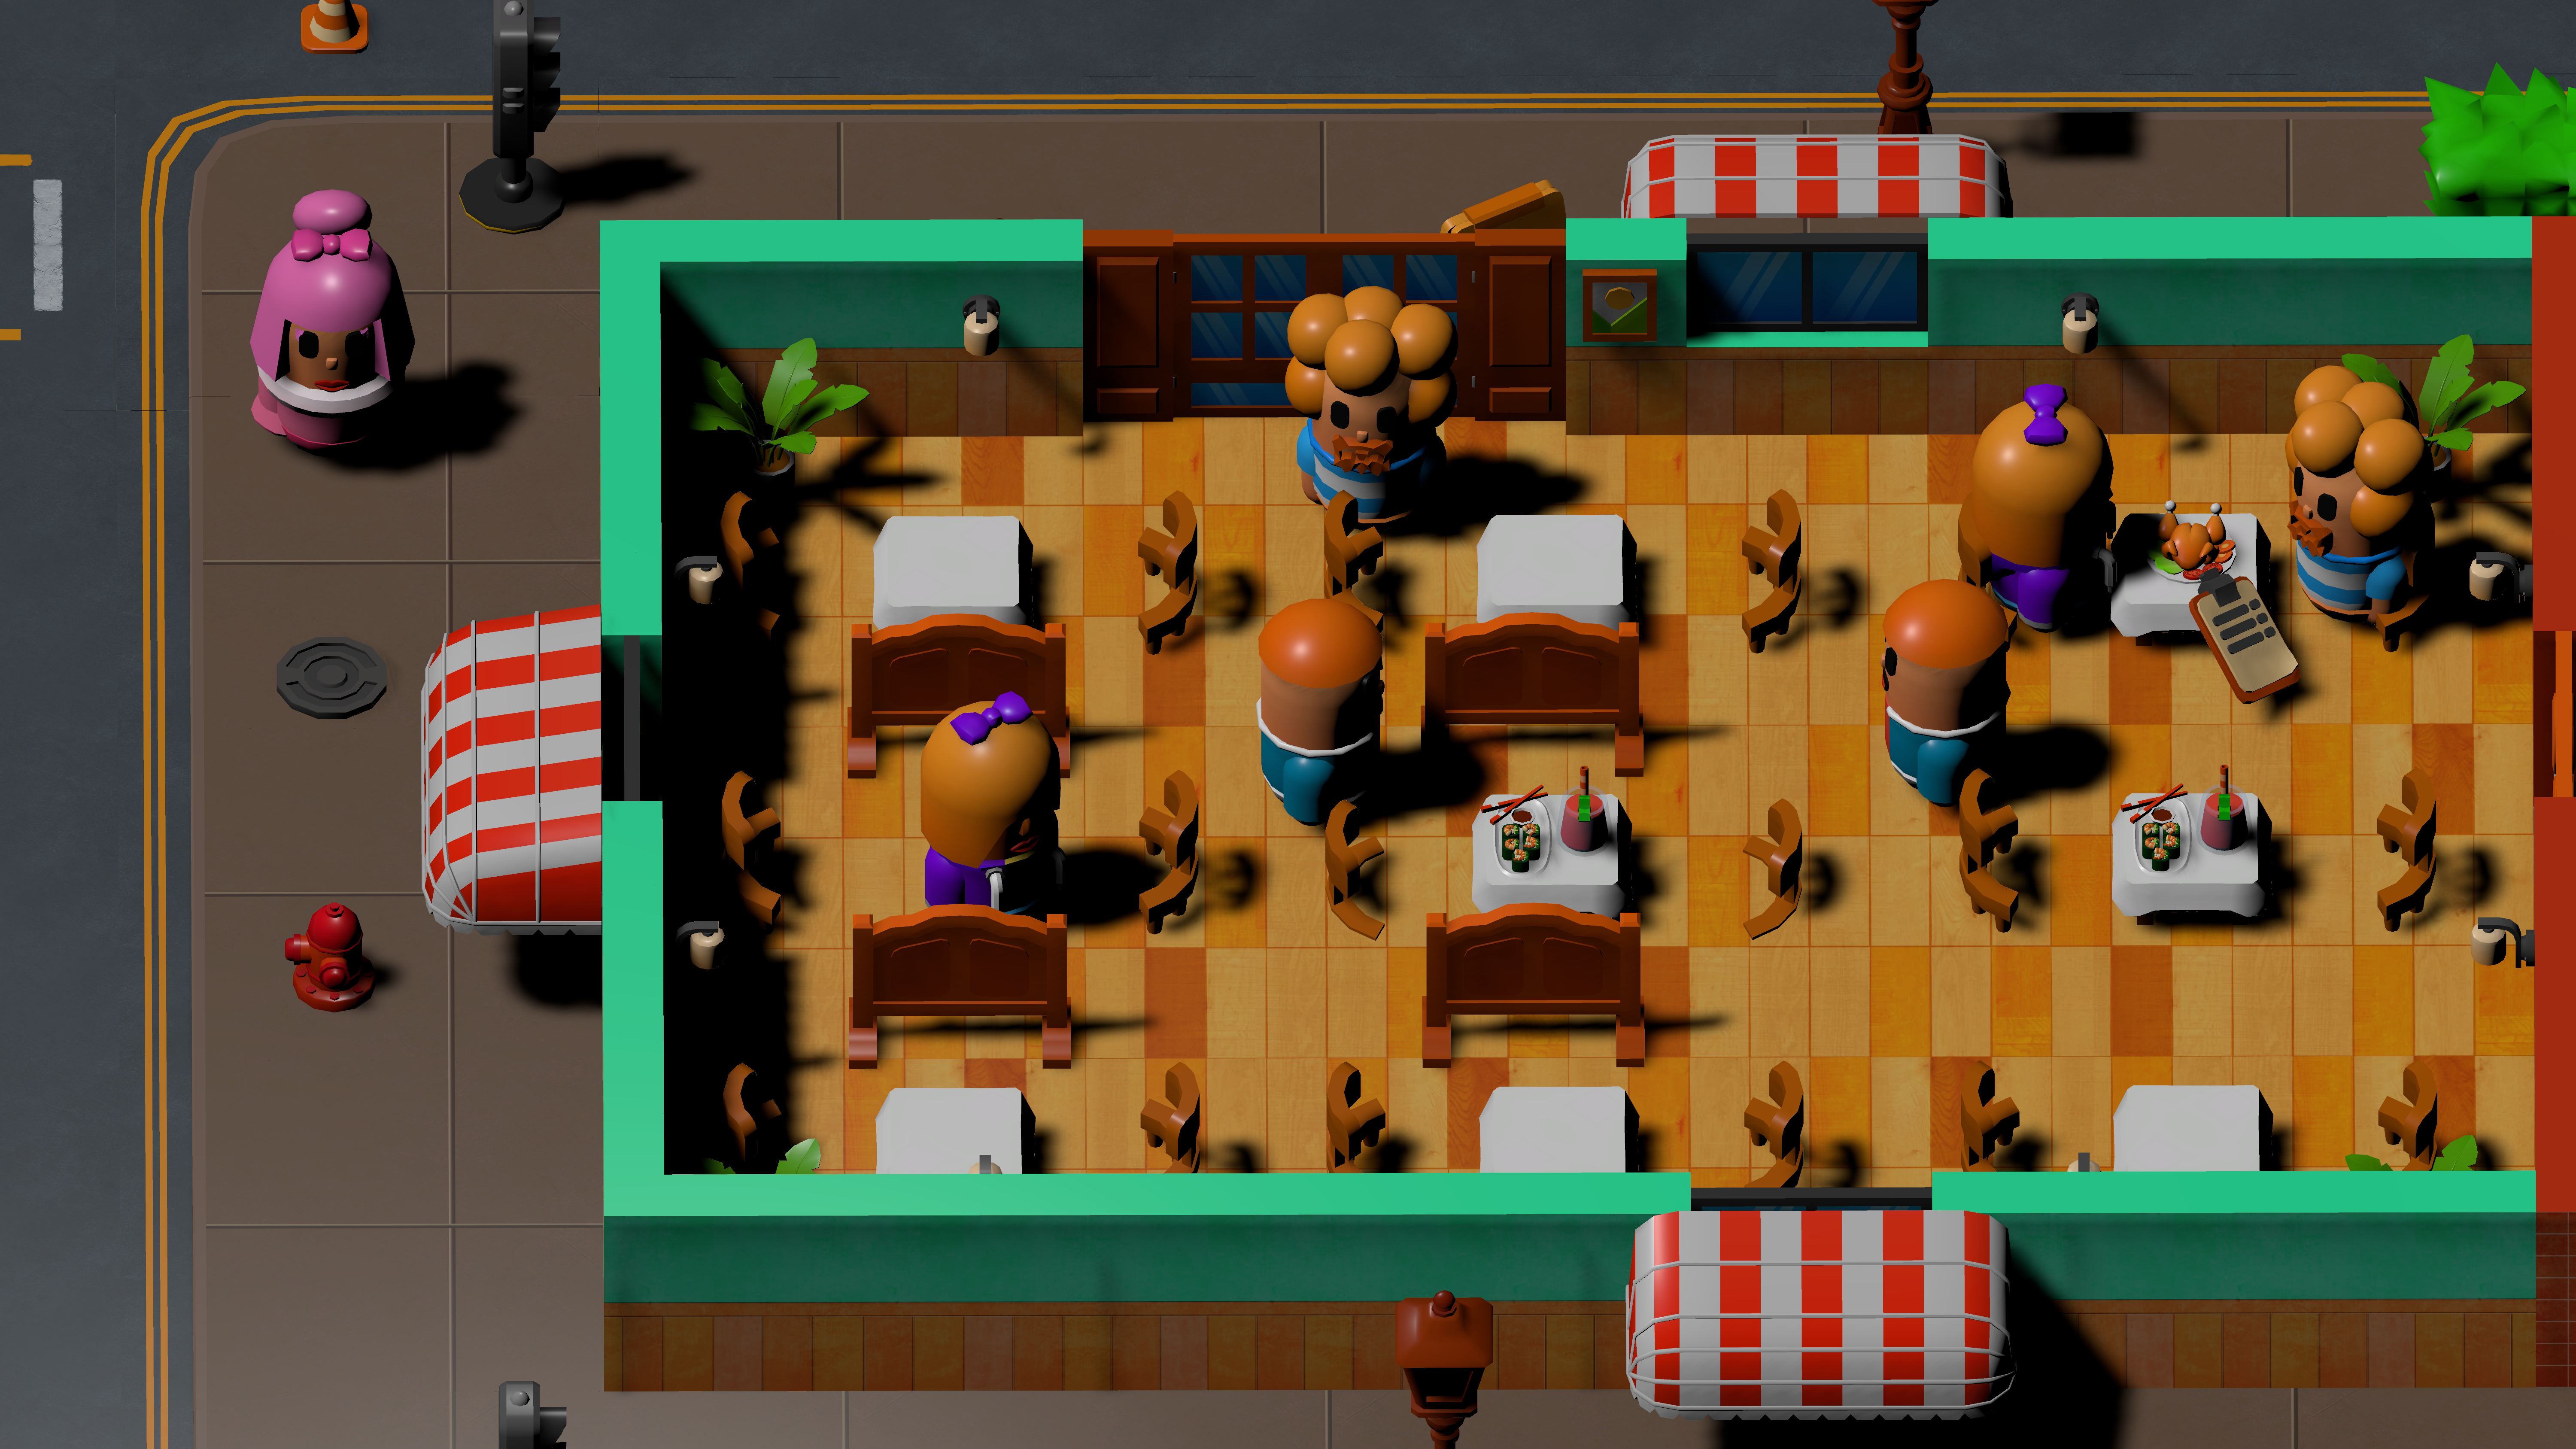
\includegraphics[width=\linewidth]{Figure_Environment_Dining_Detail.png}\caption{Dining area}\end{subfigure}\hfill
  \begin{subfigure}[b]{0.192\textwidth}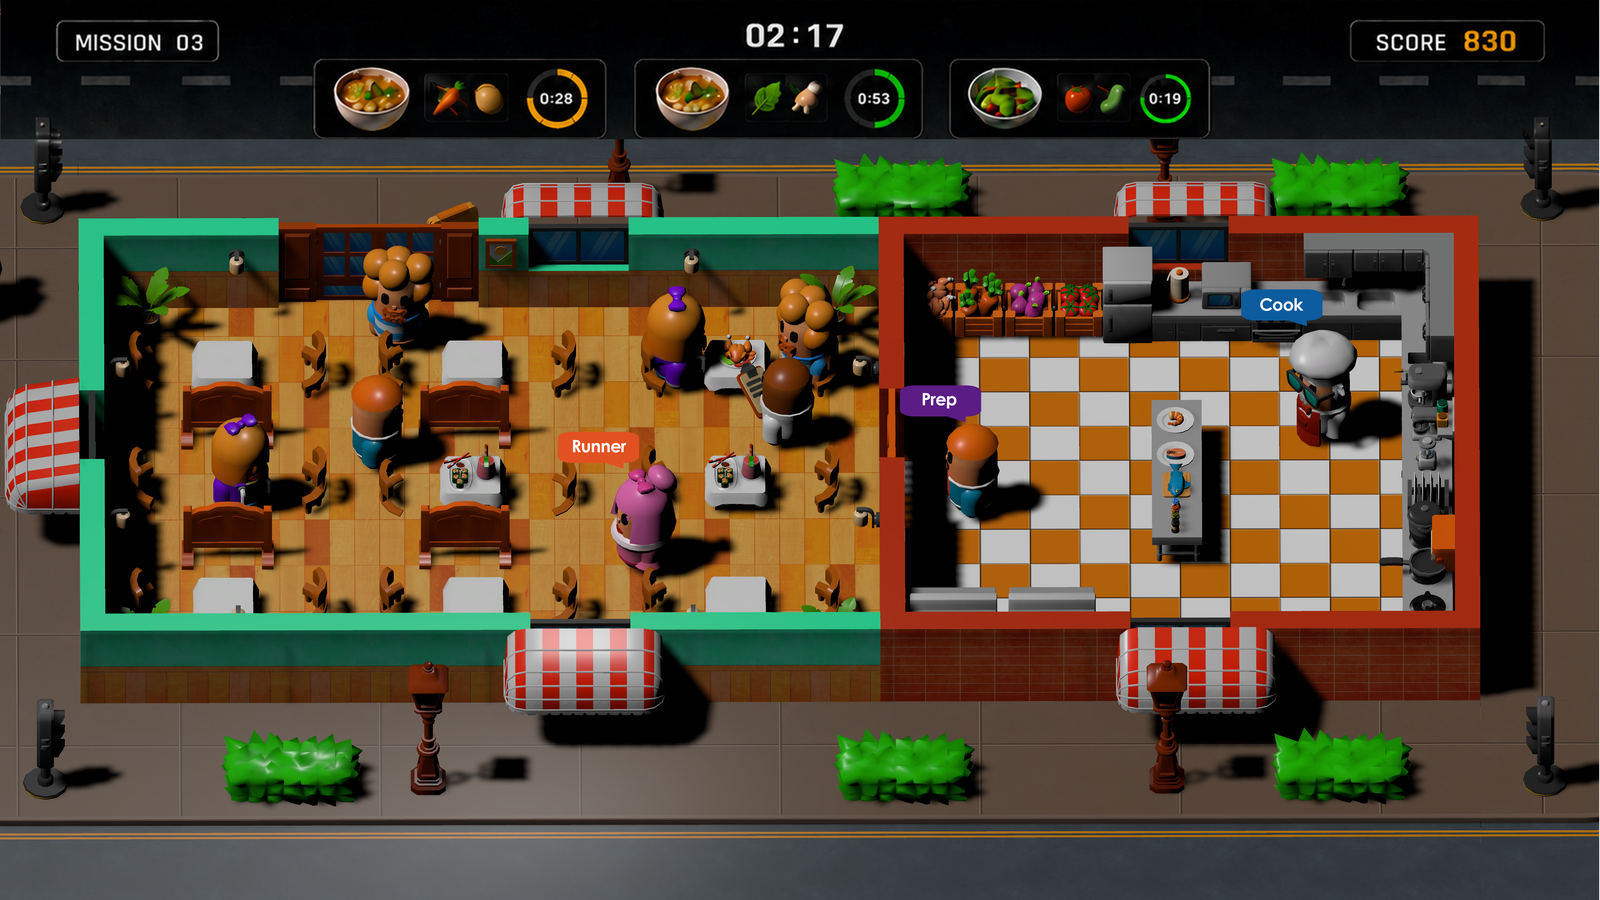
\includegraphics[width=\linewidth]{Figure_1_Teaser_NoCue.png}\caption{No Cue}\end{subfigure}\hfill
  \begin{subfigure}[b]{0.192\textwidth}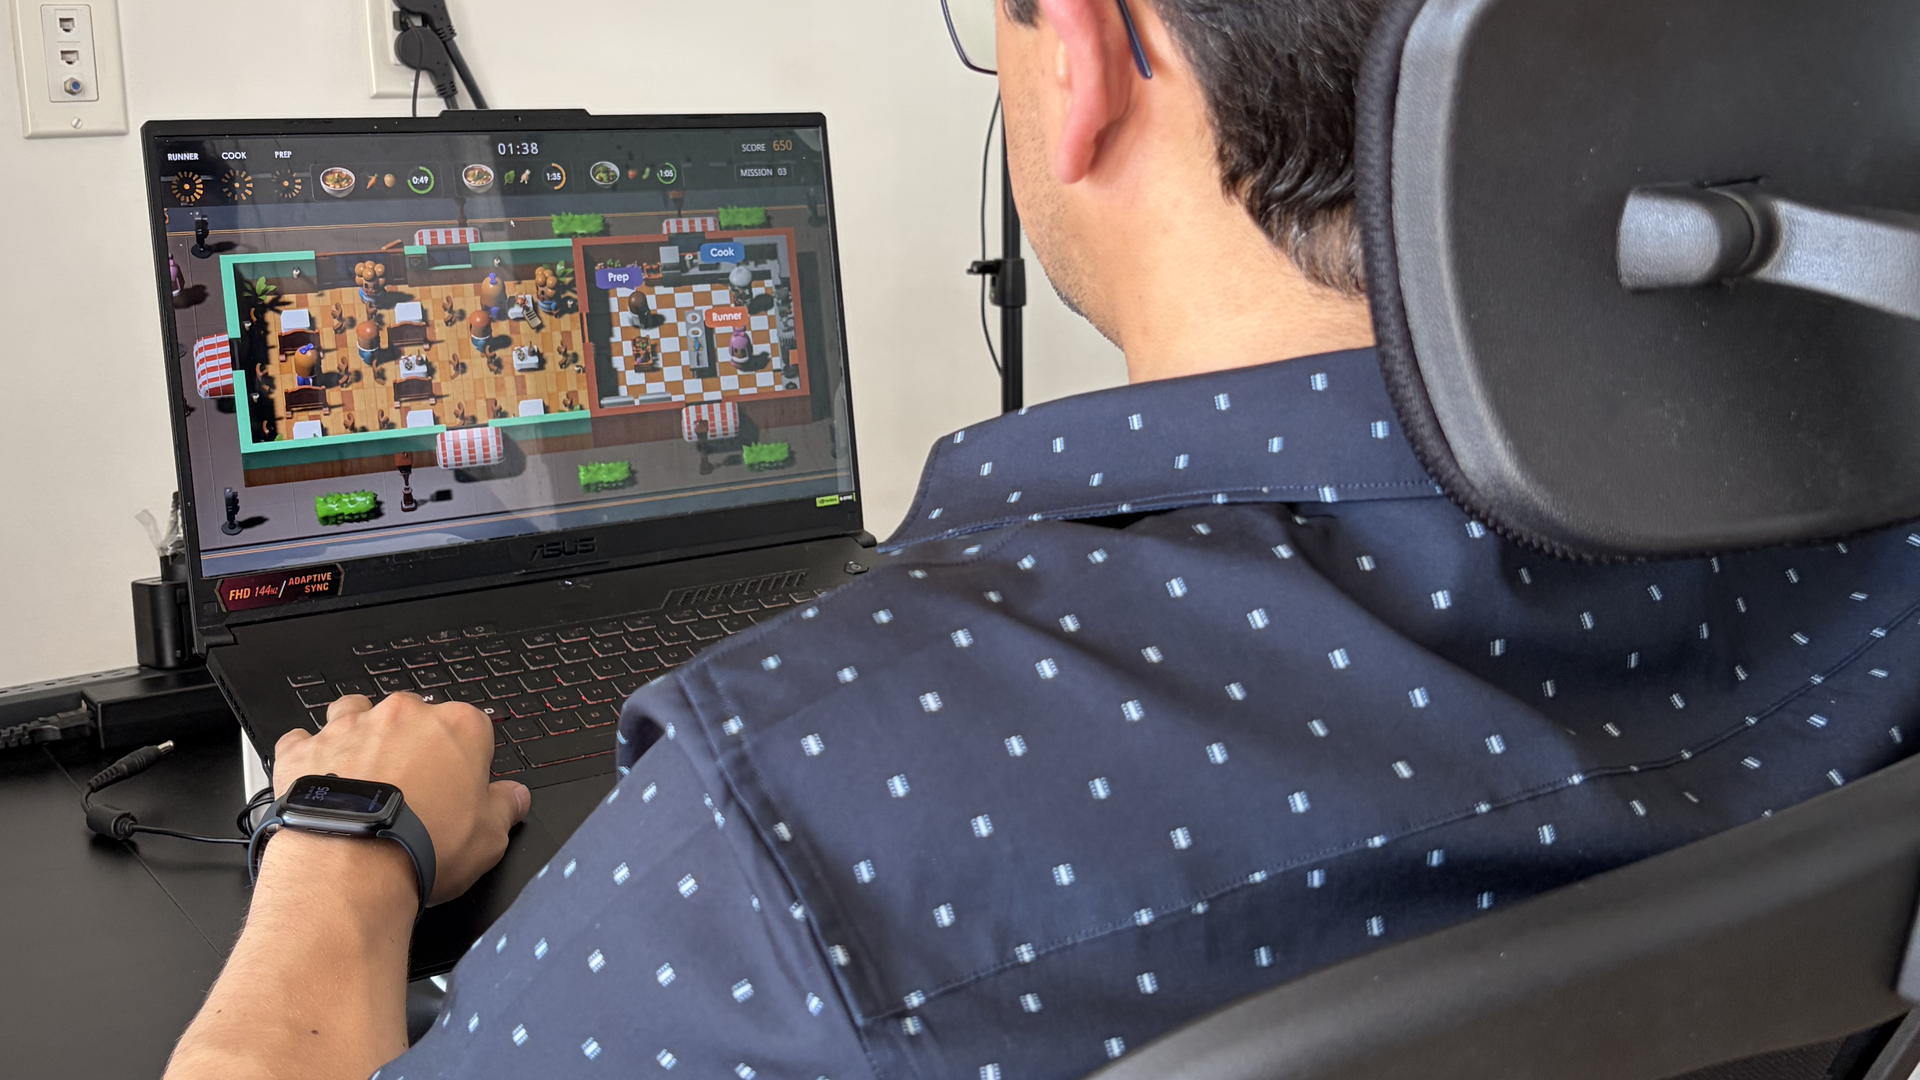
\includegraphics[width=\linewidth]{Figure_Participant_Apparatus.png}\caption{\rev{Apparatus}}\end{subfigure}\\[4pt]
  \begin{subfigure}[b]{0.49\textwidth}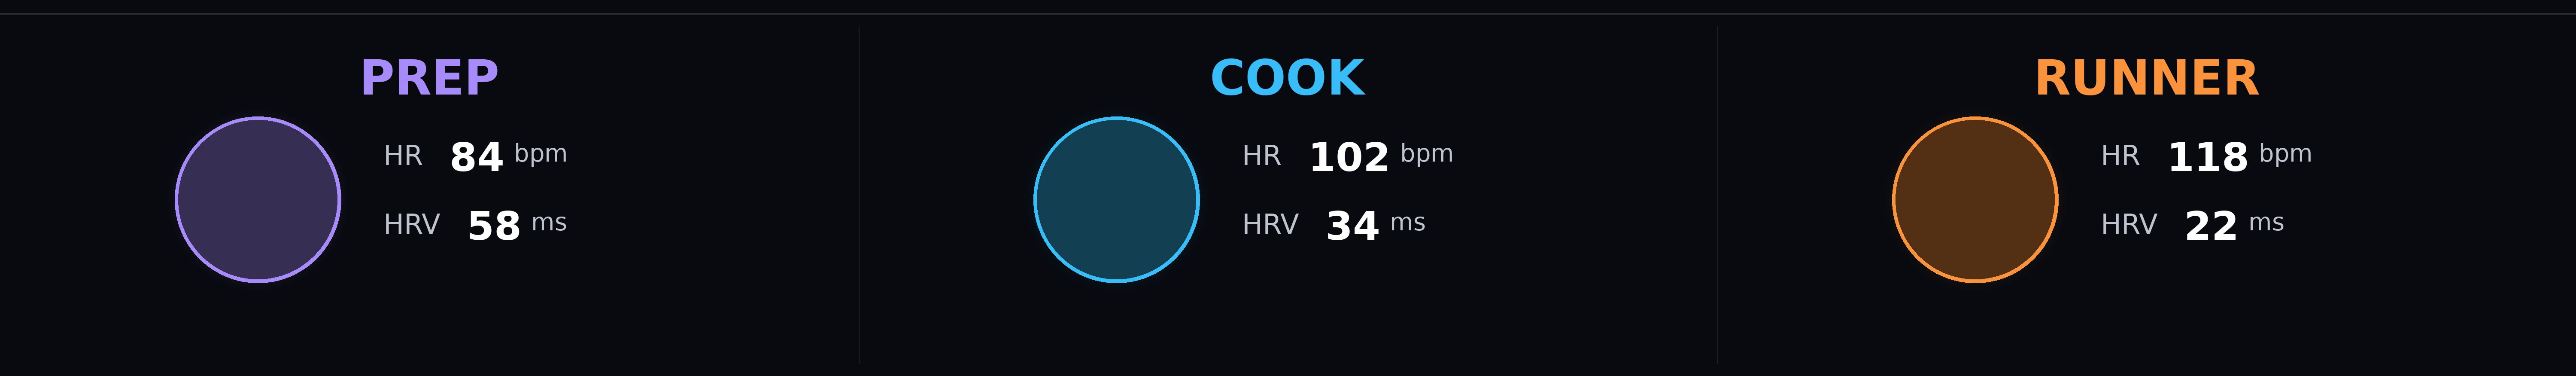
\includegraphics[width=\linewidth]{Figure_NumericCue_Detail.png}\caption{Numeric Cue}\end{subfigure}\hfill
  \begin{subfigure}[b]{0.49\textwidth}
\includegraphics[width=\linewidth]{Figure_IconCue_Detail.png}\caption{Icon Cue}\end{subfigure}
  \caption{Study~2 setup: environment overview, kitchen and dining details, the No Cue view, \rev{the participant apparatus with Apple Watch,} and the Numeric Cue and Icon Cue status bars. Panels (f) and (g) show the same illustrative values.}
  \Description{Top row: a top-down game layout, close-ups of the kitchen and dining area, the game view without a physiological overlay, and a participant seated at a computer wearing an Apple Watch. Bottom row: a status bar with HR and HRV numbers per role, and the same status bar with one glowing halo per role instead.}
  \label{fig:s2setup}
\end{figure*}

\subsection{\texorpdfstring{\revbox{Measures and Analysis}}{Measures and Analysis}}
\rev{\textbf{Support response time} was measured in seconds from actual pressure-event onset to the first relevant support action by another teammate. \textbf{Appropriate support actions} were coded separately: a support action was appropriate when it matched the immediate task need, for example passing ingredients, covering a pot, plating a dish, or delivering an order. Appropriateness was contextual rather than an intrinsic property of an action, so response time marks when support began, whereas the appropriate-support count captures whether support fit the need. Event logs recorded action type, appropriateness, prior verbal requests, and cue references. Service Rush also assessed whether appropriate support occurred within ten seconds. \textbf{Recovery time} was measured in seconds from actual pressure-event onset until the task bottleneck was resolved: the required ingredients had been prepared and supplied for both affected orders (Ingredient Bottleneck), both affected pots had been cleared (Pot Overload), or the dishes, dirty plates, and deliveries pending at event onset had been processed (Service Rush). Successful dish retrieval and burning were distinguished; newly arriving work was excluded from the Service Rush endpoint. Unresolved events were recorded as unrecovered. This measure describes task recovery, not physiological recovery.}

\rev{Behavioral outcomes were analyzed at the team-by-condition level ($n=12$ teams), using repeated-measures ANOVA and planned two-sided paired $t$ contrasts (Icon versus No Cue, Icon versus Numeric, and Numeric versus No Cue), with Cohen's $d_z$. The primary contrast was Icon versus No Cue for support response time. The 108 pressure events were nested within 12 teams, not treated as independent observations. Questionnaire comparisons used participant-by-condition paired $t$ tests ($n=36$ participants) over the same three contrasts. Analyses used Python with pandas, SciPy, and statsmodels.}

\rev{Team communication was coded post hoc into eight categories: task instructions, support offers, status checks, uncertainty statements, help requests, strategy changes, physiological references, and numeric references. Coding relied on one primary coder without a verified reliability sample. Category frequencies were compared at the team-by-condition level with Friedman tests followed by Wilcoxon signed-rank pairwise contrasts. Answers to the closing open-ended questions were coded with theme labels applied during data collection; this is distinct from Study~1's reflexive thematic analysis.}

\subsection{\texorpdfstring{\revbox{Results}}{Results}}
\textbf{Display reliability.} All 36 participants completed all missions (108 pressure events). Latency averaged 180--247\,ms, missing data 3.5--4.5\% of samples, and displayed states matched classified states on all 555 logged samples \rev{from the cue-present conditions. This agreement establishes display fidelity, not observer comprehension (Section~\ref{sec:scope}).}

\textbf{Support behavior.} Support response time was 15.3\,s under No Cue, 12.5\,s under Numeric Cue, and 11.4\,s under Icon Cue (Figure~\ref{fig:s2results}a). Icon Cue was \textbf{3.90\,s faster than No Cue} ($t(11)=-5.05$, $p<.001$, $d_z=-1.46$), and Numeric Cue was 2.87\,s faster than No Cue \rev{($t(11)=-4.49$, $p=.001$, $d_z=-1.30$)}. Icon Cue was numerically faster than Numeric Cue (11.4 vs.\ 12.5\,s), but this difference was \emph{not statistically significant} \rev{($t(11)=-1.81$, $p=.098$, $d_z=-0.52$)}. \rev{Task recovery time decreased from 29.0\,s under No Cue to 23.2\,s under Icon Cue ($t(11)=-5.31$, $p<.001$, $d_z=-1.53$). Teams logged more appropriate support actions under Numeric Cue (3.17) and Icon Cue (3.42) than under No Cue (2.25; descriptive team means, Figure~\ref{fig:s2results}d).} Uncertainty statements and help requests decreased when a cue was available, while support offers and strategy-change talk rose specifically under Icon Cue \rev{(Friedman tests, all $p<.001$; corresponding Wilcoxon contrasts, all $p\leq.002$)}.

\begin{figure*}[t]
  \centering
  \begin{subfigure}[b]{0.22\textwidth}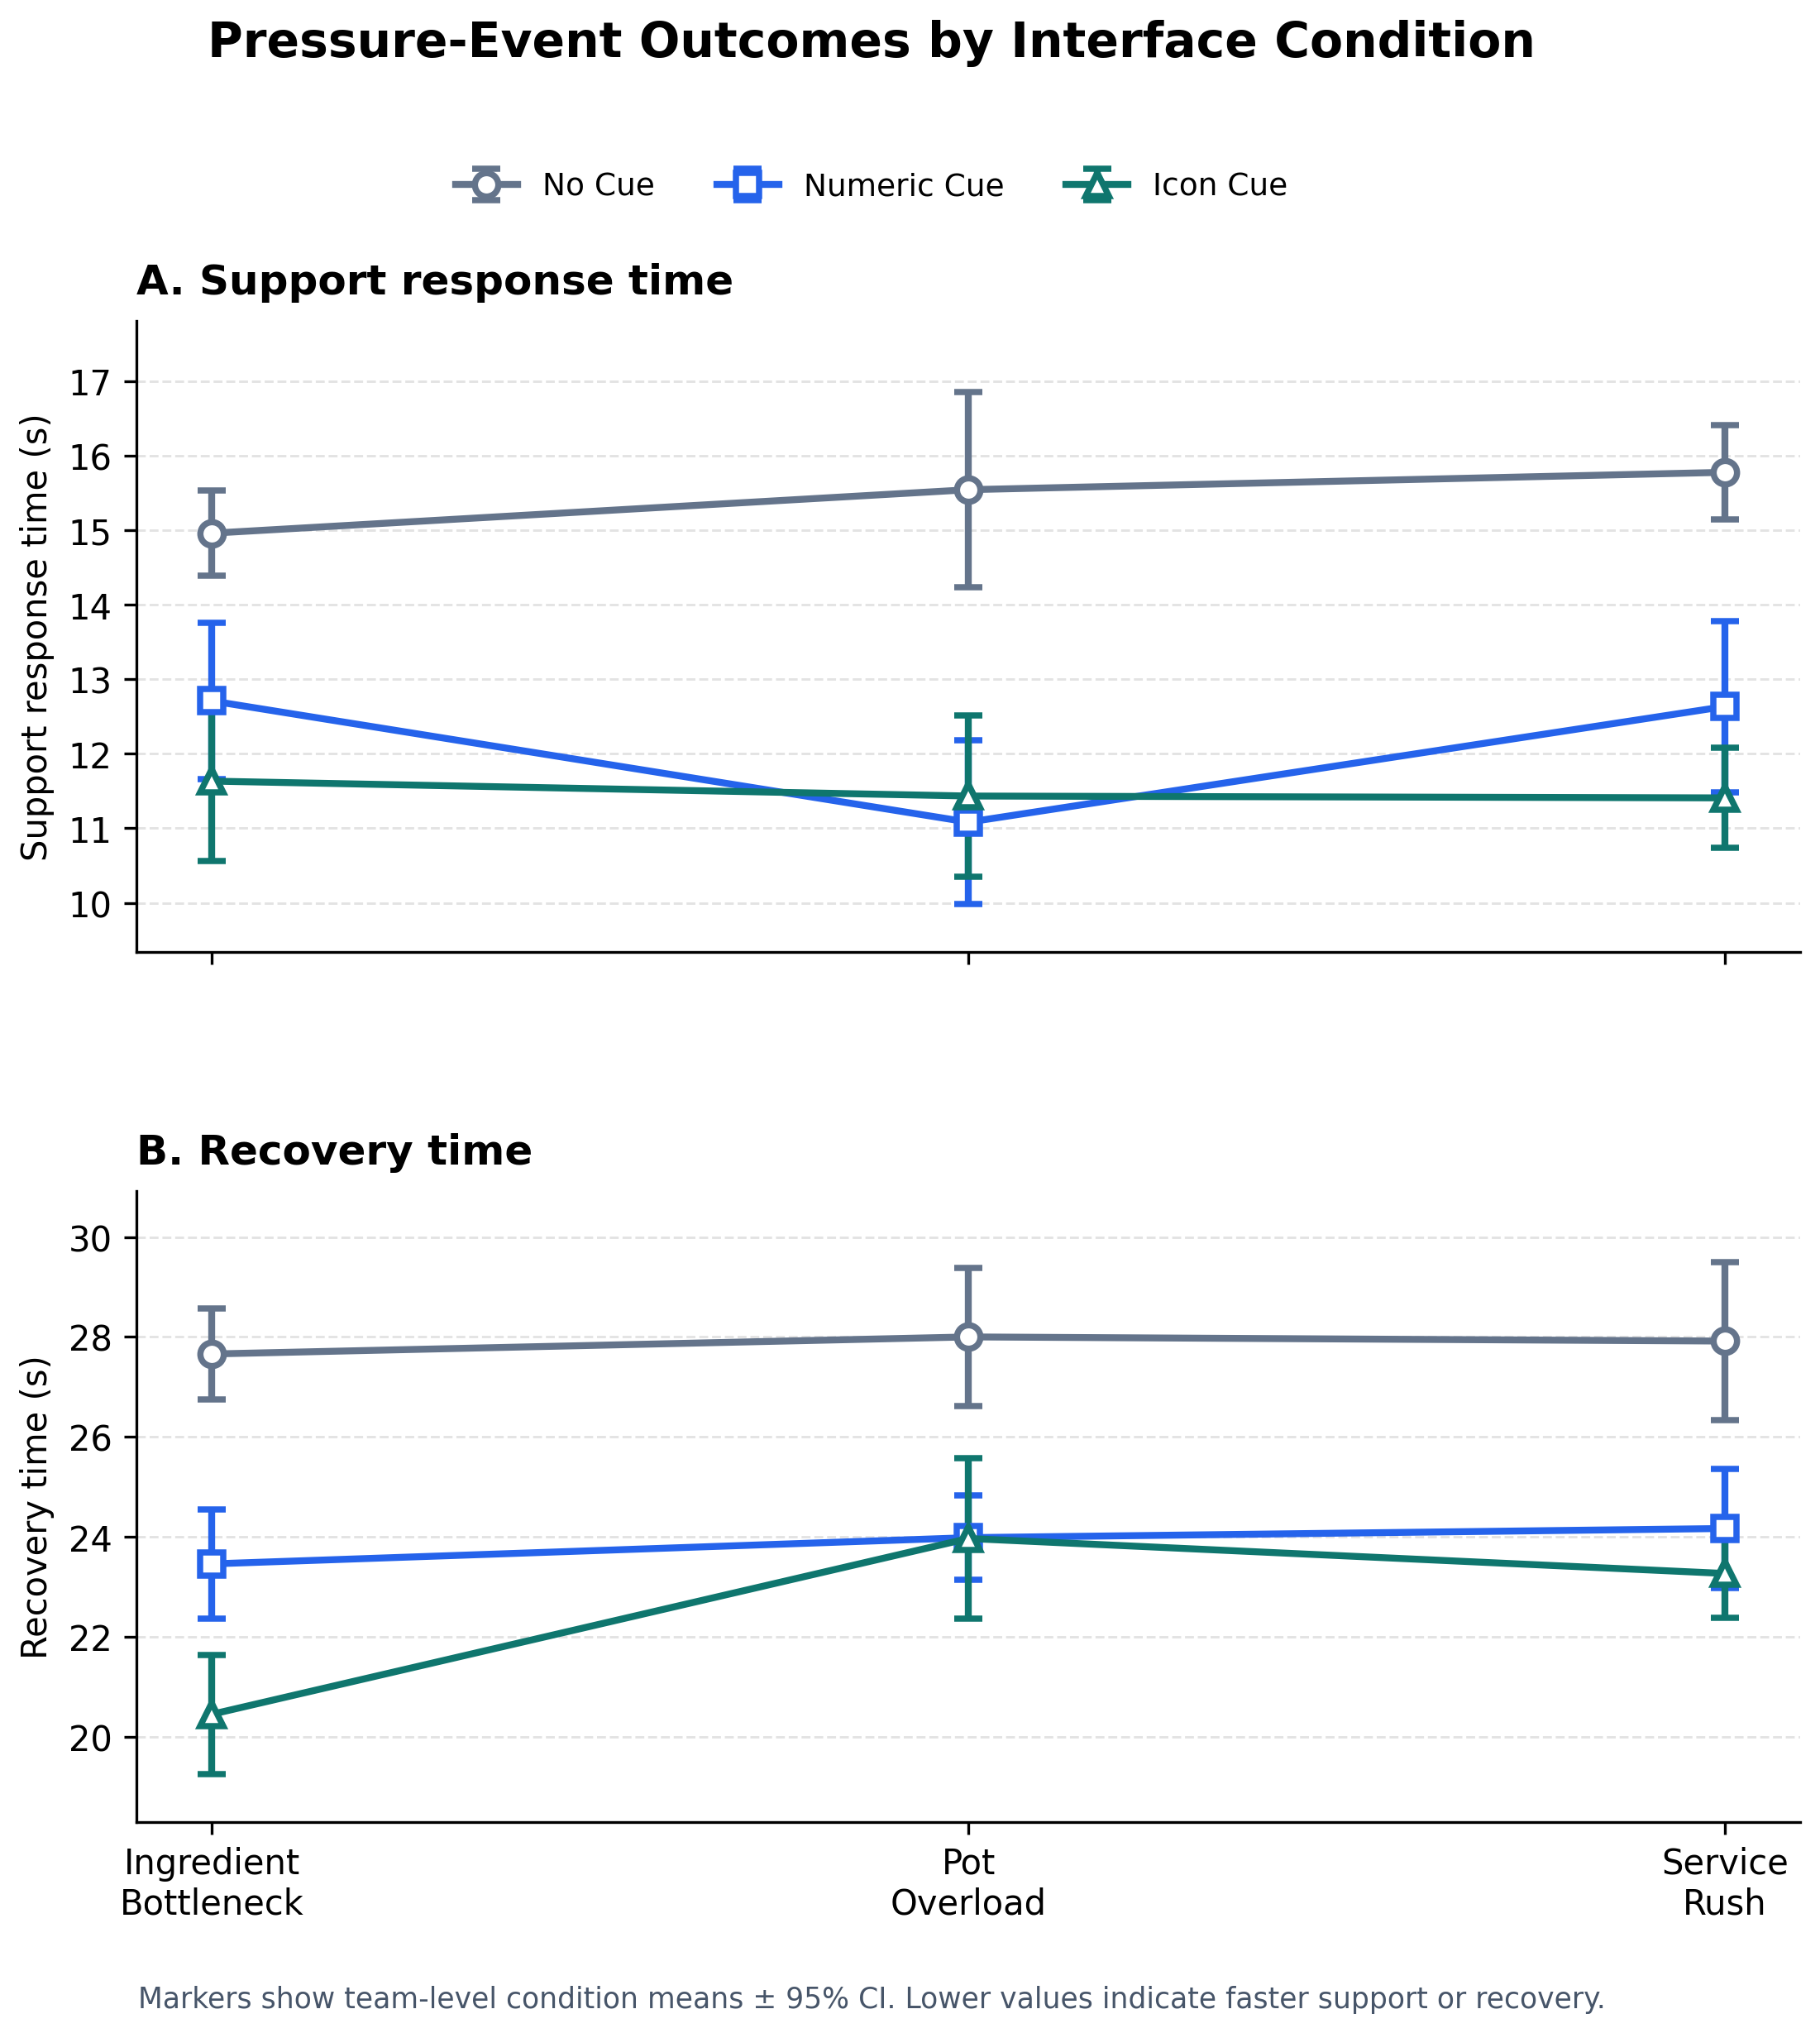
\includegraphics[width=\linewidth]{Figure_5_Pressure_Event_Breakdown_Clean.png}\caption{Support response and recovery time by pressure event.}\end{subfigure}\hfill
  \begin{subfigure}[b]{0.35\textwidth}
    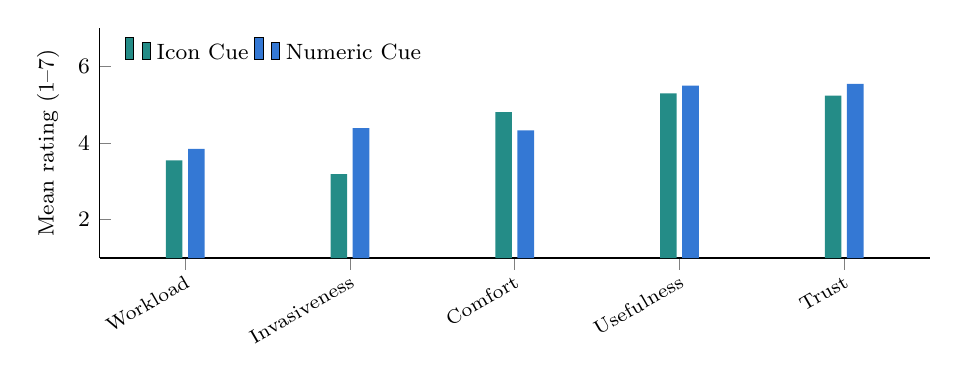
\begin{tikzpicture}
      \begin{axis}[width=\linewidth, height=4.5cm, ybar, bar width=6pt, ymin=1, ymax=7,
          symbolic x coords={Workload, Invasiveness, Comfort, Usefulness, Trust}, xtick=data,
          ylabel={Mean rating (1--7)}, axis lines*=left, enlarge x limits=0.13,
          legend style={font=\footnotesize, draw=none, at={(0.02,0.99)}, anchor=north west, legend columns=2},
          tick label style={font=\footnotesize}, label style={font=\footnotesize},
          x tick label style={font=\scriptsize, rotate=30, anchor=north east, inner sep=1pt}]
        \addplot[draw=none, fill=iconcue] coordinates {(Workload,3.55) (Invasiveness,3.19) (Comfort,4.81) (Usefulness,5.30) (Trust,5.24)};
        \addplot[draw=none, fill=numcue]  coordinates {(Workload,3.85) (Invasiveness,4.39) (Comfort,4.33) (Usefulness,5.50) (Trust,5.55)};
        \legend{Icon Cue, Numeric Cue}
      \end{axis}
    \end{tikzpicture}
    \caption{Post-condition ratings for Icon and Numeric Cue.}
  \end{subfigure}\hfill
  \begin{subfigure}[b]{0.40\textwidth}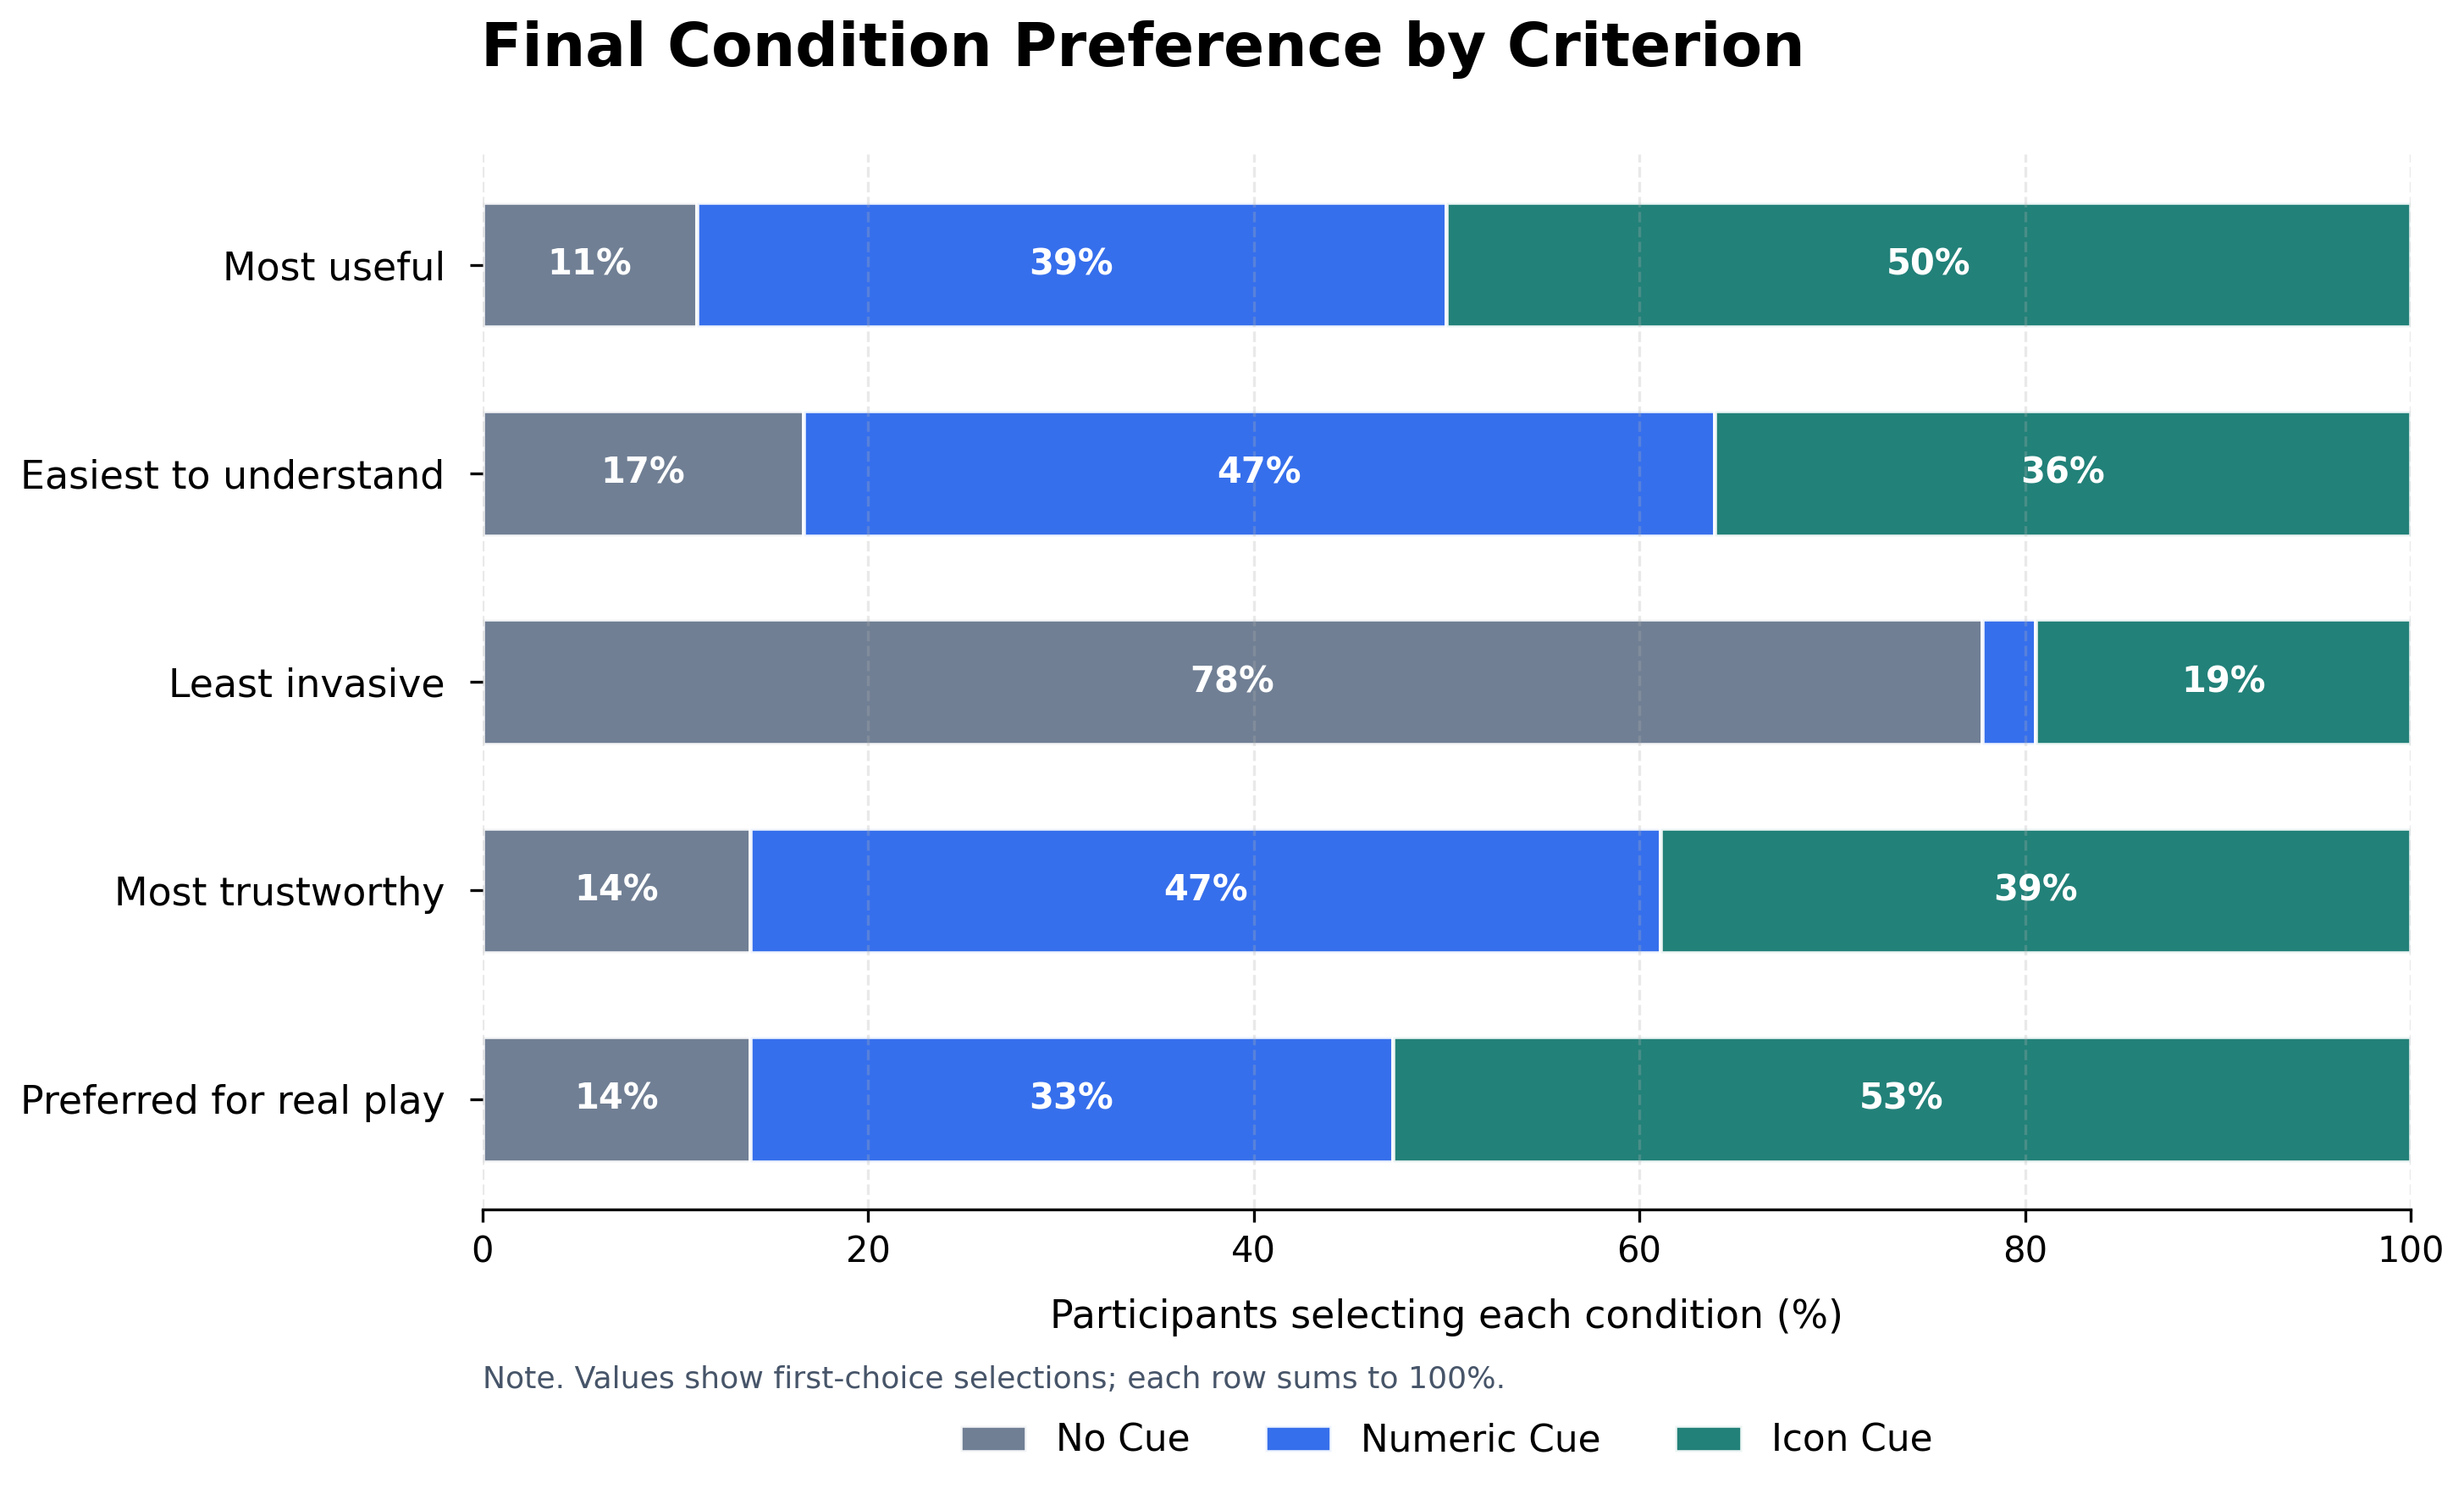
\includegraphics[width=\linewidth]{Figure_10_Final_Condition_Preference_Final.png}\caption{Final first-choice preferences by criterion.}\end{subfigure}\\[6pt]
  \begin{subfigure}[b]{0.86\textwidth}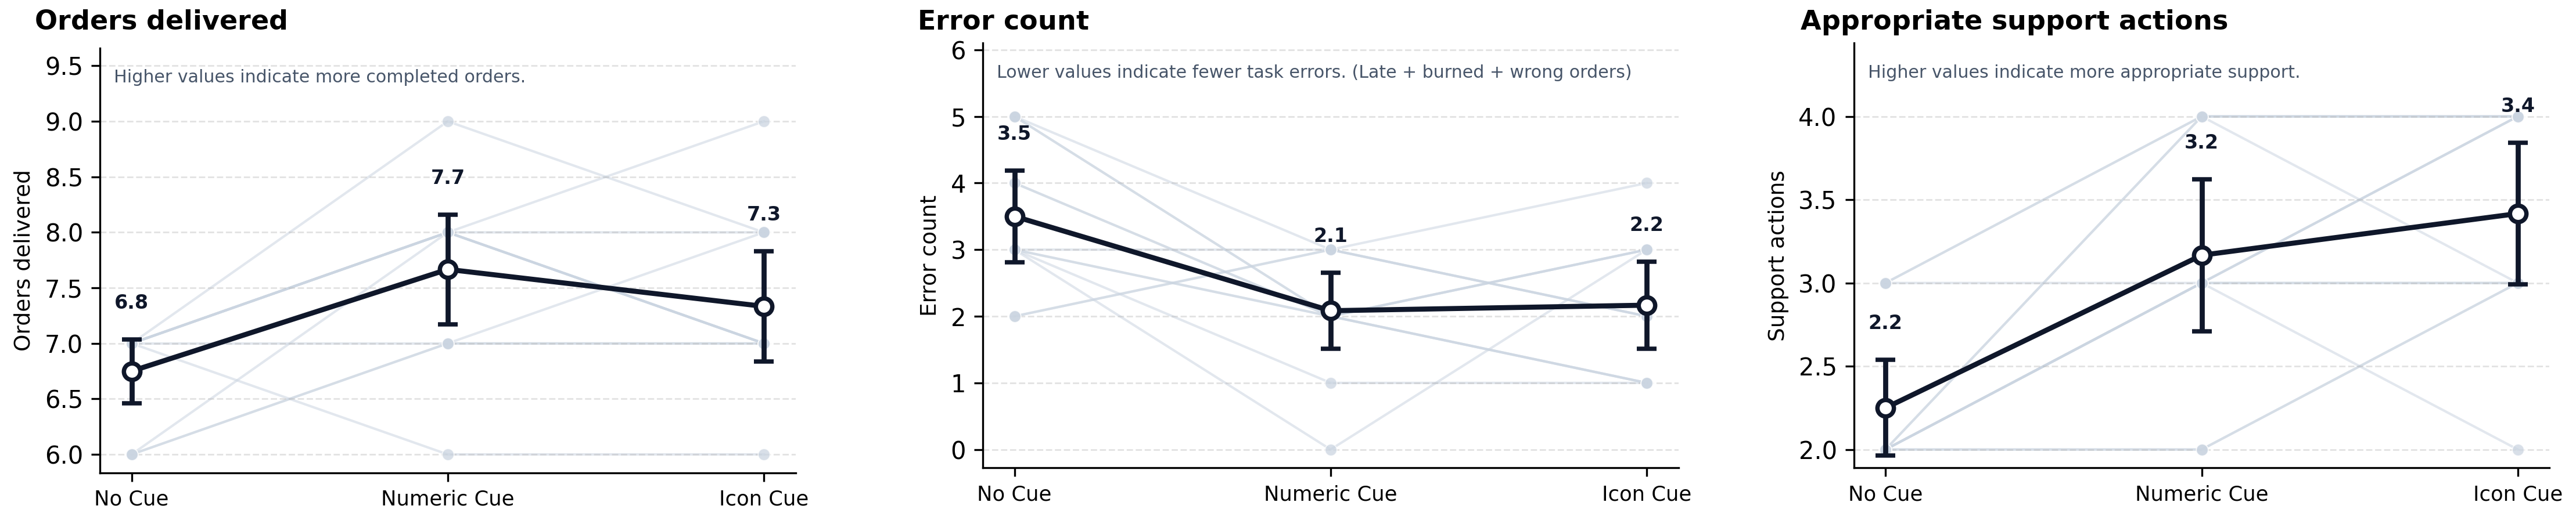
\includegraphics[width=\linewidth]{Figure_6b_Team_Performance_Panels.png}\caption{\rev{Team performance: orders delivered, error count, and appropriate support actions.}}\end{subfigure}
  \caption{Study~2 results: \rev{(a) support response and task recovery by pressure event; (b) post-condition ratings; (c) final preferences; and (d) orders delivered, errors, and appropriate support actions. In (d), gray lines show team-level means and black markers show condition means $\pm$ 95\% CI.}}
  \Description{Four panels: support response and recovery time by pressure event for the three conditions; paired bars for Icon Cue versus Numeric Cue on workload (3.55 vs 3.85), perceived invasiveness (3.19 vs 4.39), comfort sharing (4.81 vs 4.33), coordination usefulness (5.30 vs 5.50), and trust (5.24 vs 5.55); stacked bars of first-choice preferences by criterion; and line charts of orders delivered, error count, and appropriate support actions across No Cue, Numeric Cue, and Icon Cue.}
  \label{fig:s2results}
\end{figure*}

\textbf{Awareness, workload, and perceived invasiveness.} Teammate awareness rose from 4.21 under No Cue to 5.34 under Icon Cue ($p<.001$), \rev{with no statistically significant difference from Numeric Cue} (5.42; $p=.49$). Workload was lower under Icon Cue than Numeric Cue (four-item descriptive mean 3.55 vs.\ 3.85, $p=.004$). \rev{The four-item workload mean had low internal consistency (Cronbach's $\alpha=.13$) and should be interpreted descriptively rather than as a validated composite.} Perceived invasiveness was lower under Icon Cue than Numeric Cue (3.19 vs.\ 4.39, $p<.001$), though higher than under No Cue (2.11), and comfort sharing was higher (4.81 vs.\ 4.33, $p=.013$). \rev{Numeric Cue was rated higher on coordination usefulness (5.50 vs.\revcs 5.30, $p=.023$) and trust (5.55 vs.\revcs 5.24, $p=.002$)} (Figure~\ref{fig:s2results}b).

\textbf{Final preferences.} Final preferences revealed a complementary pattern: 50\% selected the Icon Cue as most useful and 53\% preferred it for real cooperative play, whereas 47\% selected the Numeric Cue as easiest to understand and 47\% as most trustworthy; 78\% selected No Cue as least invasive (Figure~\ref{fig:s2results}c). Participants therefore distinguished between an ambient cue they preferred in play and exact values they trusted for interpretation: ``The icon felt more like part of the game; the numbers felt like a measurement tool. The trade-off was speed versus precision'' (P042).

%% =====================================================================
\section{\texorpdfstring{\revbox{Discussion and Limitations}}{Discussion and Limitations}}
Study~1 shows that the label-free encoding is readable well above chance; Study~2 shows that the same encoding can influence team behavior during live cooperative play. \rev{No statistically significant difference in teammate awareness was detected between Icon and Numeric Cue. Icon Cue had lower reported workload and perceived invasiveness, but Numeric Cue scored higher on coordination usefulness and trust.} The result is therefore not a clean advantage for ambiguity. Instead, it suggests a hybrid design in which an ambient cue remains the default and exact values are surfaced when greater specificity is useful. We frame this as a design implication of these findings: \textbf{default to ambience, and reveal precision when needed}. Participants repeatedly asked for optional, mutable visibility, motivating \textbf{opt-in sharing}, an \textbf{immediate off switch}, and \textbf{separate permissions for ambient icons and exact numeric values}. Because each halo is driven by only two classified values, the same architecture could also support shared displays, tabletops, or spectator walls \cite{morrisonsmith_ambiteam_2021}; whether bystanders read the cue differently from teammates remains untested.

\rev{\textbf{What the scripted events do and do not show.}}\label{sec:scope} \rev{The two studies support different claims. Study~1 tested \emph{recognition}: whether viewers could identify the intended HR and HRV state of isolated halos. In Study~2, \emph{physiological input was live}, but the \emph{task-pressure events were scripted}; event onset is the behavioral timing reference and does not establish a particular physiological response in the overloaded player. Agreement between \emph{displayed and classified states} shows that the halo rendered what the classifier produced. It does not show that teammates \emph{understood the intended cue information} during a given event: Study~2 included no event-specific comprehension check. Faster assistance under a cue may therefore also reflect visible task difficulty in the shared game view or verbal communication, not the physiological information alone.}

\rev{\textbf{Collaborative XR spaces.} Avatar placement in social AR is sensitive to the available physical space and meeting context \revcite{drago_exploring_2025}, while digital-proxemics research examines how display and audio affordances relate to personal space, proximity, and attention in virtual collaboration \revcite{williamson_digital_2022}. These findings motivate studying avatar-associated physiological halos in collaborative AR/VR rather than assuming that a fixed desktop HUD transfers unchanged: where a halo is placed relative to an avatar or seat, how proximity and attention change its visibility, and who in a shared space may see it. A future evaluation could compare HUD-based and spatially anchored cues during joint tasks, measuring cue interpretation, support response, workload, and perceived invasiveness while examining proximity, occlusion, and audience-specific sharing permissions. This is a proposed extension: the current desktop-game studies do not establish effectiveness in XR.}

\textbf{Limitations.} Recognition accuracy was moderate, and middle states were harder to separate than the endpoints. Study~2 used one wearable ecosystem, scripted pressure events, short missions, and 12 team-level units without an a priori power analysis for team-level comparisons, so the nonsignificant Icon--Numeric difference is not evidence of equivalence. \rev{The reported results do not establish that teammates correctly interpreted the physiological cue during individual scripted pressure events. Communication was coded by a single primary coder without a verified reliability sample.} Both studies used convenience samples, and consent and data ownership remain open questions.

%% =====================================================================
\section{Conclusion}
Across two independent samples, a wearable-driven, label-free physiological cue made remote teammates' HR/HRV states readable above chance and accelerated support relative to No Cue. Compared with explicit numerical disclosure, the Icon Cue \rev{showed no statistically significant difference from Numeric Cue in teammate awareness, with lower workload and perceived invasiveness, while Numeric Cue yielded higher coordination usefulness and trust.} These findings position ambient physiological cues as a complementary, privacy-sensitive layer for distributed coordination rather than a replacement for precise physiological information.

\subsection{\texorpdfstring{\revbox{Ethics / Data / AI Use}}{Ethics / Data / AI Use}}
\textbf{Ethics.} Both studies were approved under a single institutional ethics board approval before data collection. Participants gave informed consent and could withdraw or stop physiological sharing at any time; HR and HRV data were used for research and interface visualization only, not diagnosis, and were stored under coded participant identifiers. \textbf{Data.} Anonymized data, stimuli, and analysis scripts will be released upon publication. \textbf{AI use.} \rev{Generative AI tools (ChatGPT and Claude Code) were used for language editing and restructuring of author-drafted text. During this revision, ChatGPT also assisted with identifying related literature, and Claude Code assisted with LaTeX formatting and checking reference metadata. These tools were not used to generate participant data or reported statistical results. The authors verified all sources, reviewed the final text, and take responsibility for it.}

\clearpage
\bibliographystyle{ACM-Reference-Format}
\bibliography{references}

\end{document}
